\documentclass[11pt,a4paper,UTF8,fontset=windows]{ctexart}
\usepackage[margin=2.2cm]{geometry}
\usepackage{amsmath,amssymb,graphicx,booktabs,tabularx,array,float,caption,xcolor}
\usepackage[section]{placeins}
\usepackage{longtable}
\usepackage[numbers,sort&compress]{natbib}
\usepackage[colorlinks=true,linkcolor=blue!45!black,citecolor=blue!45!black,urlcolor=blue!45!black]{hyperref}
\graphicspath{{figures/}}
\captionsetup{font=small,labelfont=bf}
\setlength{\parskip}{3pt}
\setlength{\emergencystretch}{2em}
\renewcommand{\arraystretch}{1.15}
\newcolumntype{Y}{>{\raggedright\arraybackslash}X}
\title{\textbf{VOLT-KD：面向轻量多标签心电图分类的\\幅值保留学习}}
\author{}
\date{}
\begin{document}
\maketitle
\vspace{-2em}
\begin{abstract}
轻量心电图分类需要在有限计算预算下保留有效的诊断信息。逐记录、逐导联标准化在统一信号尺度的同时消除了绝对电压及导联幅值比例，使幅值相关信息在进入网络前发生改变。针对这一问题，本文提出幅值保留的轻量多标签分类框架 VOLT-KD。该框架以毫伏信号为输入，通过多尺度深度可分离卷积和短序列建模形成紧凑表征，并利用诊断子类与交叉拟合的基础模型软标签进行训练。教师及辅助头仅在训练期使用，部署学生包含 107,189 个参数。PTB-XL 上的五种子实验表明，同一学生采用毫伏输入后，宏平均 ROC-AUC 从 0.9106 提高至 0.9277，肥厚类别 ROC-AUC 从 0.8285 提高至 0.9019；第二种紧凑骨干呈现一致改善。完整框架达到宏平均 ROC-AUC $0.9298\pm0.0012$ 和宏平均 F1 $0.7542\pm0.0009$，较 MSCA-Mamba 文献报告均值分别提高 0.0300 和 0.0504。在已有子类监督的学生上，蒸馏将宏平均 F1 进一步提高 0.0043，且保持部署网络规模。电压探针、增益响应和诊断子类分析共同支持输入幅值的作用；分组、多强度扰动、概率质量及近期文献比较进一步刻画完整流程的性能。模型估计运算量为 30.1 MFLOPs，在测试平台上的单线程 CPU 推理延迟为 32.5 ms。该研究将诊断信息保留、紧凑表征与训练期知识学习相结合，为轻量心电图分类提供了具有可解释依据的设计方案。
\end{abstract}
\noindent\textbf{关键词：}心电图；多标签分类；幅值保留；轻量网络；知识蒸馏

\section{引言（Introduction）}
十二导联心电图多标签分类旨在从同一段心电信号中同时识别正常心电图、心肌梗死、ST/T 改变、传导异常和肥厚等诊断类别，是自动心电图分析的重要任务\cite{wagner2020}。与只判断一种异常的二分类不同，多标签分类需要同时处理异常共存、类别分布不均衡以及不同疾病线索相互重叠的问题。一段十秒记录中，局部波形反映形态变化，跨心搏关系提供时间信息，不同导联的电压及其比例则描述空间分布。面向资源受限设备，这些信息必须在有限存储和计算预算下转化为有效预测。因此，轻量化的目标既包括压缩网络，也包括提高有限模型对输入诊断信息的利用效率。PTB-XL 提供的患者独立分折和分层诊断标签，为研究这一问题建立了统一的数据基础\cite{wagner2020}。

现有研究主要从特征提取与信息融合提高分类能力。以 MSCA-Mamba\cite{cetintas2026} 为例，其处理流程先将每条记录的每个导联标准化，再使用多尺度卷积提取局部形态，通过通道重标定和状态空间模块整合特征，最后输出多个诊断概率。该方法以 121,149 个参数取得宏平均 ROC-AUC 0.8998，说明紧凑网络可以完成这一任务。Chimera\cite{behrouz2024} 从状态空间建模出发，增强时间及变量之间的动态依赖表达；MS-LTCAF\cite{feng2025} 通过导联—时间协同注意力选择关键观测位置；DBA-ASFNet\cite{luo2025} 结合深度可分离残差卷积、双向 GRU 与年龄、性别信息，降低表征学习开销；CNN--FFT\cite{malik2026} 则将时域形态与频域特征融合。这些工作对网络内部的信息提取给出了不同答案。相较之下，进入网络之前的幅值处理与后续类别收益之间，仍需要建立明确的实验联系：当预处理将波形映射到统一尺度时，被移除的尺度究竟是干扰，还是模型本应保留的诊断内容？

这一问题在肥厚识别中具有直接意义。Sokolow--Lyon 和 Cornell 等电压指标都由特定导联的波幅构成\cite{sokolow1949,casale1985,hancock2009}。逐记录、逐导联 z-score 使不同绝对幅值的同形波形获得近似相同表示，同时改变导联之间的幅值比例。网络仍可利用形态和标签共现关系进行分类，但物理电压已不再以原有形式参与学习。已有 DeepECG 研究也将幅值处理纳入基础模型的预处理设计\cite{nolin2026}。本文关注的进一步问题是：在约十万参数的紧凑分类器中，保留毫伏尺度能够带来多大的收益，这种收益集中在哪些类别，又是否在不同骨干中保持一致？围绕该问题建立对照，有助于把预处理从固定默认步骤转化为有任务依据的模型设计。

另一条研究路线是在训练阶段增加知识。ECGFounder\cite{li2025} 通过超过一千万条心电记录学习诊断表征，ECG-FM\cite{mckeen2025} 提供开放的自监督基础模型；MVKT-ECG\cite{qin2023} 利用多视图知识迁移，将多导联教师的信息传递给单导联学生。这些研究拓展了小模型可利用的监督来源，但教师整体分数、类别能力与学生输入表示之间的关系仍值得针对性评价。大模型的高总体性能并不意味着每个诊断类别都向学生提供同样有利的目标。与此同时，PTB-XL 的二十三个诊断子类和高采样率记录提供了比五个大类硬标签更丰富的训练信息。如何在保持轻量推理的同时组织这些信息，并辨别输入保留与额外监督各自的作用，构成本文的第二个设计问题。

针对上述问题，本文提出幅值保留的轻量多标签分类框架 VOLT-KD，将物理输入、紧凑表征和训练期知识学习组织为连续的分类流程。输入端将记录转换为毫伏，仅去除导联常量偏移，使电压差异直接进入特征提取；网络端利用多尺度深度可分离卷积与下采样提取波形模式，再由短序列上的双向 GRU 聚合上下文；训练端结合大类硬标签、子类硬标签和基础模型软标签。教师软标签通过交叉拟合生成，使每条训练记录对应于未使用其所属微调折的教师。额外诊断子类和高采样率教师均限定在训练阶段，部署时只保留 100 Hz 输入、学生骨干及五类预测头。本文沿用成熟的卷积、循环与蒸馏组件，将创新重点放在幅值保留的任务化设计，以及输入、监督和计算预算之间可检验的联系上。

VOLT-KD 具有三个相互衔接的特点。首先，信息保留作用于学习流程的起点：同一学生仅改变输入处理，宏平均 ROC-AUC 即从 0.9106 提高到 0.9277，HYP 从 0.8285 提高到 0.9019。其次，推理规模由紧凑骨干控制：完整学生部署参数为 107,189，估计运算量为 30.1 MFLOPs，完整配置达到宏平均 ROC-AUC 0.9298 和宏平均 F1 0.7542。最后，额外监督的作用通过固定学生的组件比较明确，蒸馏在已有子类监督上进一步提高宏平均 F1。为评价这一组合，本文同时给出近期文献参照、同协议模型比较、诊断子类与人群分组、概率质量、合成扰动及推理效率；这些分析分别回答整体水平、增益来源、类别覆盖和资源收益问题。

本文的贡献概括如下：
\begin{enumerate}
\item 提出面向紧凑多标签心电图分类的幅值保留学习流程，将毫伏输入与多尺度时序表征结合。通过无需训练的电压探针、两个骨干的输入对照和增益响应，把输入中保留的信息、模型性能及预测行为联系起来，解释肥厚相关类别的主要收益。
\item 构建训练与部署分离的分层知识学习框架，将诊断子类和交叉拟合教师概率用于共享骨干训练，部署时保留单一轻量预测通路。阶梯与移除式分析量化了输入设计的主要作用，并确定教师软标签对宏平均 F1 的增量贡献及类别差异。
\item 在 PTB-XL 上验证约十万参数的单学生可取得较高多标签分类性能，并保持较低运算量与较高批量吞吐。诊断子类、测试亚组、输入扰动和减导联结果进一步刻画该设计在不同观测条件下的性能与资源权衡。
\end{enumerate}

VOLT-KD 将诊断信息保留、紧凑特征提取与训练期知识学习结合，使有限的推理容量能够利用物理电压和多层次监督。
\section{相关工作（Related Work）}
\subsection{紧凑心电图分类网络}
紧凑网络通过卷积、注意力和序列模块在有限参数下提取心电图特征。MSCA-Mamba 采用多尺度卷积、SE 注意力和单向状态空间模块，以约十二万参数完成多标签分类\cite{cetintas2026}。这一路线重点优化不同时间尺度的特征提取和聚合。本文继承多尺度建模思想，以深度可分离卷积和下采样降低特征提取及后续序列处理的开销，并将物理幅值作为输入设计的重要因素。两者在预处理和骨干内部计算方式上的差异，为本文的输入对照与效率评价提供了直接比较对象。

近期方法进一步拓展了这一方向。Chimera 以二维状态空间结构建模动态时间与变量关系\cite{behrouz2024}，MS-LTCAF 对导联及时间位置进行协同加权\cite{feng2025}。DBA-ASFNet 已采用深度可分离卷积与双向 GRU，并融合人口信息\cite{luo2025}；本文使用这些成熟组件构造紧凑学生，重点研究幅值输入及训练监督的组合。CNN--FFT 通过确定性频域分支补充时域表征\cite{malik2026}。这些路线表明，紧凑分类的性能既依赖计算结构，也依赖送入结构的信息种类。本文从物理电压这一信息来源出发，以受控输入对照连接设计与结果。

\subsection{预训练表征与知识迁移}
自监督学习利用大规模心电信号建立可迁移表征。Mehari 与 Strodthoff 研究了十二导联自监督学习对标签效率与噪声条件下性能的影响\cite{mehari2022}；HeartBEiT 通过图像式心电图预训练支持下游诊断\cite{vaid2023}。ECGFounder 在超过一千万条记录上进行监督预训练\cite{li2025}，ECG-FM 则构建开放的自监督心电图基础模型\cite{mckeen2025}。这些研究为利用历史数据中的诊断知识提供了基础。

将大模型知识迁移到轻量学生，可使预训练资源服务于资源受限推理。Qin 等的 MVKT-ECG 使用多视图知识迁移和多标签蒸馏，将多导联信息传递给单导联学生\cite{qin2023}。本文关注固定十二导联输入下的轻量分类，通过五个诊断大类、二十三个诊断子类和教师概率共同组织训练目标。教师输入为 500 Hz，学生输入为 100 Hz，额外监督集中于训练阶段。相同学生的组件比较进一步说明这些监督对整体指标与不同类别的作用。Mert 等近期比较研究将卷积、状态空间、循环、时频变换和 ECGFounder 微调纳入同一五类任务，并以异构集成进一步提高分数\cite{mert2026}。本文以其单模型和集成结果作为不同推理配置的文献参照，评价轻量单模型的性能位置。

\subsection{幅值处理与诊断信息保留}
心电图信号中的幅值既受采集条件影响，也包含诊断相关信息。近年的 DeepECG 研究将幅值范围处理纳入跨来源预处理，并系统评价基础模型的外部表现与效率\cite{nolin2026}。该工作为保留幅值的处理原则提供了当代研究背景。本文进一步将这一原则落实到约十万参数的分类器，以电压探针刻画输入差异，用两个紧凑骨干验证实际分类收益，并用教师—学生比较揭示监督的类别作用。由此，幅值处理从一个预处理选项转化为可以通过模型行为和分类结果检验的设计因素。

\section{方法（Method）}
\subsection{任务定义与总体框架}
给定一段十秒十二导联记录，学生输入为 $X\in\mathbb R^{12\times1000}$，对应 100 Hz 采样率，输出五个诊断大类的独立概率 $p\in[0,1]^5$。二元标签 $y\in\{0,1\}^5$ 允许共现，涵盖正常心电图（NORM）、心肌梗死（MI）、ST/T 改变（STTC）、传导异常（CD）和肥厚（HYP）。训练时同时使用二十三个子类标签 $u\in\{0,1\}^{23}$。

VOLT-KD 由幅值保留预处理、轻量学生骨干和训练期分层监督组成（图\ref{fig:framework}）。毫伏输入保留波形电压，多尺度卷积与短序列建模提取紧凑特征，大类标签、子类标签和 ECGFounder 教师概率共同监督学生训练。推理阶段删除教师和子类辅助头，仅保留学生骨干及五类预测头。
\begin{figure}[htbp]
\centering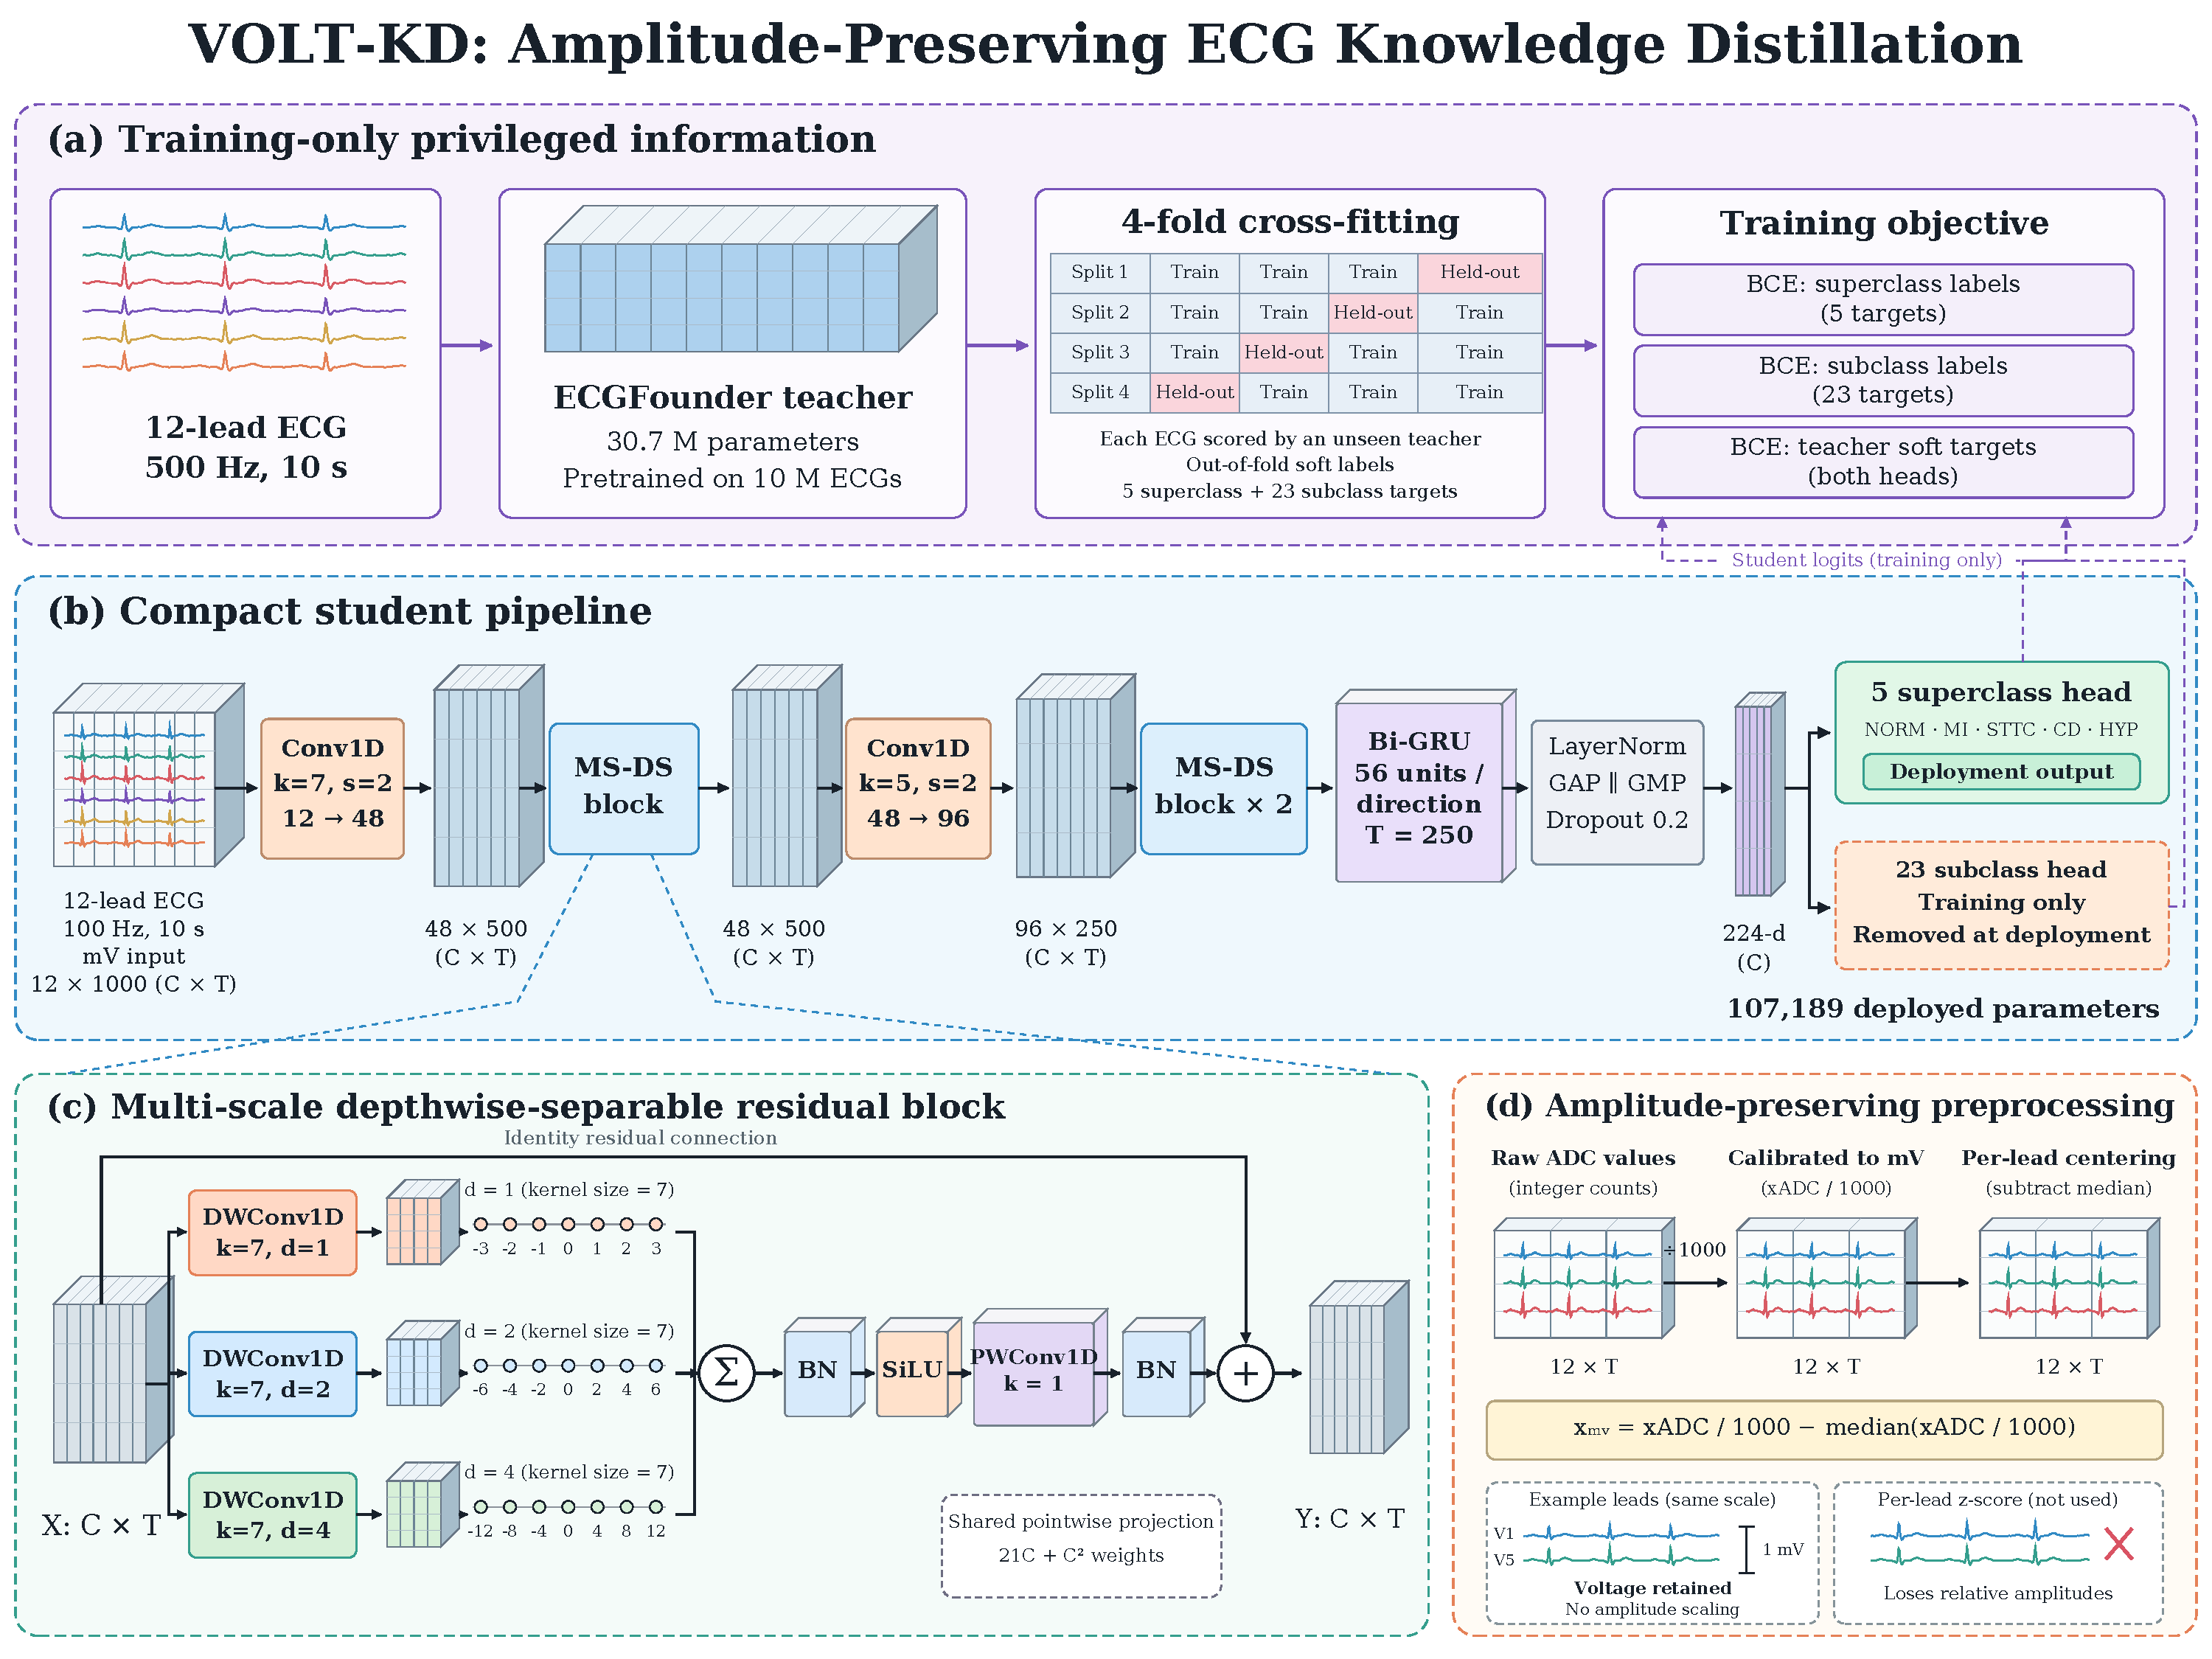
\includegraphics[width=\linewidth]{f02_architecture.pdf}
\caption{幅值保留的训练与推理流程。高采样率记录、教师软标签和诊断子类只在训练阶段使用；推理阶段输入为 100 Hz 心电图，输出为五个诊断大类。完整 VOLT-KD 使用大类、子类与教师监督。}
\label{fig:framework}
\end{figure}

\subsection{物理幅值保留}
幅值处理的设计出发点是区分常量偏移与波形电压。对单条记录的第 $\ell$ 个导联，逐导联标准化写为
\begin{equation}
 Z_\ell(X)=\frac{X_\ell-\mu_\ell}{s_\ell+\epsilon},
\end{equation}
其中 $\mu_\ell$、$s_\ell$ 由该记录自身计算，$\epsilon=10^{-6}$。忽略稳定项且 $s_\ell>0$ 时，对于正增益 $a_\ell$ 和常量偏移 $b_\ell$，有
\begin{equation}
 Z_\ell(a_\ell X_\ell+b_\ell)=Z_\ell(X_\ell).
\end{equation}
这意味着不同绝对幅值的同形信号被映射到相同表示。标准化统一了输入尺度，也使这一尺度本身退出了后续学习过程。

为保留该信息，本文按记录的存储增益将 ADC 值转换为毫伏，再减去每个导联的时间中位数：
\begin{equation}
 \widetilde X_\ell(t)=X^{\mathrm{ADC}}_\ell(t)/1000
 -\operatorname{median}_{\tau}\big(X^{\mathrm{ADC}}_\ell(\tau)/1000\big).
\end{equation}
常数 1000 对应本次 PTB-XL 数据的 ADC 增益。该操作去除常量偏移，并保持波形的毫伏幅值；导联之间和记录之间的电压差异由后续网络处理。输入没有逐记录尺度除法，训练与推理使用相同处理步骤。

\subsection{多尺度紧凑时序表征}
不同持续时间的心电图形态需要不同的时间感受野。本文采用膨胀率为 1、2、4 的三个深度卷积分支提取多尺度特征，并共享逐点投影以控制通道混合的计算开销\cite{howard2017}。分支卷积核均为 7，输出相加后依次通过批归一化、SiLU、逐点卷积和批归一化，与输入形成残差连接。对 $C$ 个通道，不计偏置与归一化参数，权重数为 $21C+C^2$；三个完整卷积分支则为 $21C^2$。这一计算形式将时间尺度扩展与通道混合分开，使多尺度提取保持较小的参数量。

骨干先以核为 7、步长为 2 的卷积将十二导联映射到 48 通道，再经过一个多尺度块。第二级采用核为 5、步长为 2 的卷积，扩展至 96 通道，并连接两个多尺度块。两次下采样把序列长度从 1000 压缩到 250，降低后续时序建模的处理长度。每方向 56 个隐单元的双向 GRU\cite{cho2014} 聚合上下文，层归一化后的特征同时经过全局平均池化和最大池化。二者拼接后，通过丢弃率为 0.2 的 dropout 输入两个独立线性头，分别预测五个大类和二十三个子类。

训练网络包含 112,364 个参数，其中子类头包含 5,175 个参数。删除该头后，部署网络为 107,189 个参数。辅助监督通过共享骨干影响五类预测，部署模型保持单一学生通路。

\subsection{训练期分层知识学习}
五类标签提供主要任务目标，二十三个子类提供更细粒度的诊断描述。本文以独立大类头和子类头组织这两层监督，各头采用二元交叉熵。教师选用 ECGFounder\cite{li2025}，以 500 Hz 记录微调同样的二十八个目标。该设置把高采样率教师的输出用于 100 Hz 学生训练，实现额外信息在训练阶段的利用。

为构建留出软标签，将训练折 1--8 分成四组，每组包含两折。四个教师分别在其余六折微调，并对被留出的两折生成 logits。每条学生训练记录对应的教师均未在微调时使用其所属患者。教师使用整条记录跨时间和导联的均值、标准差进行标准化；此处理保留导联幅值比例。每个教师训练八轮，使用 AdamW，批量为 64、权重衰减为 $10^{-2}$，one-cycle 峰值学习率为 $3\times10^{-4}$，检查点由验证折 9 选择。

记学生大类与子类 logits 为 $z^s,z^u$，教师输出为 $t^s,t^u$，完整损失为
\begin{align}
 \mathcal L={}&\operatorname{BCE}(z^s,y)+\operatorname{BCE}(z^u,u)\nonumber\\
 &+\operatorname{BCE}(z^s,\sigma(t^s))+\operatorname{BCE}(z^u,\sigma(t^u)).
\end{align}
前两项保持学生与诊断标签的一致性，后两项通过教师概率提供软监督\cite{hinton2015}。BCE 使用 logits 实现，各项分别对批内样本和对应头的类别取均值，权重均为 1，温度为 1。两头独立预测，子类标签通过共享特征参与学习。交叉拟合使训练软标签满足患者微调折留出约束。

\subsection{电压探针与模型响应分析}
本文将输入信息与模型行为分为两个层次进行分析。第一层使用无需训练的电压探针，直接评价预处理前后电压统计量的判别能力；第二层在训练后的模型上施加增益变化，观察预测是否响应幅值。

电压探针采用 Sokolow--Lyon 与 Cornell 形式\cite{sokolow1949,casale1985}。以中心化记录的第 99 百分位数近似 R 波幅度 $R_\ell$，以第 1 百分位数的相反数近似 S 波深度 $S_\ell$，计算
\begin{equation}
 V_{\mathrm{SL}}=S_{V1}+\max(R_{V5},R_{V6}),\qquad
 V_{\mathrm C}=R_{aVL}+S_{V3}.
\end{equation}
分别在毫伏与标准化输入上计算这些统计量，评价其对 LVH 子类和 HYP 大类的 ROC-AUC。探针采用十秒整段分位数定义，阳性目标为数据库的心电图读图标签。增益实验则对测试波形乘以给定倍率，固定标签、模型参数及验证阈值，测量预测概率和阳性比例的变化。

\section{实验与结果（Experiments and Results）}
\subsection{数据与实验设置}
采用 PTB-XL 1.0.3\cite{wagner2020}，该版本包含 21,799 条记录、18,869 名患者。排除 411 条缺少诊断标签的记录后，按照官方患者独立分折使用折 1--8 训练、折 9 验证、折 10 测试。三部分分别包含 17,084、2,146 和 2,158 条记录。表\ref{tab:data}给出各类样本分布。训练与测试均涵盖五个诊断大类，标签共现由多标签目标处理。
\begin{table}[htbp]
\centering\small
\caption{PTB-XL 1.0.3 的诊断任务划分。括号内为记录级阳性比例；标签可以共现。}\label{tab:data}
\begin{tabularx}{\linewidth}{Yrrr}
\toprule
类别 & 训练集 & 验证集 & 测试集 \\
\midrule
NORM & 7596 (44.46\%) & 955 (44.50\%) & 963 (44.62\%) \\
MI & 4379 (25.63\%) & 540 (25.16\%) & 550 (25.49\%) \\
STTC & 4186 (24.50\%) & 528 (24.60\%) & 521 (24.14\%) \\
CD & 3907 (22.87\%) & 495 (23.07\%) & 496 (22.98\%) \\
HYP & 2119 (12.40\%) & 268 (12.49\%) & 262 (12.14\%) \\
记录数 & 17,084 & 2,146 & 2,158 \\
\bottomrule
\end{tabularx}

\end{table}

学生训练二十四轮，使用 AdamW\cite{loshchilov2019}，批量为 64、权重衰减为 $10^{-2}$，one-cycle 峰值学习率为 $4\times10^{-3}$，上升阶段占总步数的 15\%，梯度范数上限为 2。增强包括随机循环平移、逐记录 0.9--1.1 倍增益和标准差为 0.01 个输入单位的高斯噪声。评价采用指数移动平均权重，名义衰减为 0.999，每四步更新并进行初期修正。验证集宏平均 ROC-AUC 用于检查点选择，各类阈值在 0.05--0.95、步长 0.01 的网格中按验证 F1 选择。

主实验采用种子 42、123、456、789 和 2025，报告均值与样本标准差。宏平均 ROC-AUC 评价类别排序，宏平均平均精确率（Macro AP）评价精确率—召回率表现，宏平均 F1 评价固定阈值的分类决策。AP 使用平均精确率定义。表\ref{tab:effects}的区间由相同种子的指标差计算，描述固定测试集上的训练随机性；多项比较按探索性效应估计报告。

VOLT-KD 的输入与监督对照固定学生骨干、数据划分和训练配方，结构消融仅改变指定模块。仅大类监督配置使用五类硬标签，大类与子类监督配置增加子类目标，完整配置进一步引入 ECGFounder 教师软标签。跨骨干输入验证采用本地 MSCA-Mamba 实现，批量为 16，学习率和权重衰减均为 $10^{-4}$，最多训练三十轮，早停耐心为七轮。毫伏输入采用中位数中心化，z-score 输入采用均值中心化和标准差缩放；学生的噪声增强在各自输入单位下施加。输入对照评价这两套预处理及其增强的整体效果。主对比采用 MSCA-Mamba 文献报告值，输入对照、测试扰动、亚组及效率分析采用本地实现的预测与测量结果。
\subsection{与已有方法的整体性能比较}
VOLT-KD 在约十万参数的部署规模下同时改善了多标签排序与分类决策（表\ref{tab:main}）。其宏平均 ROC-AUC 为 $0.9298\pm0.0012$，高于 MSCA-Mamba 文献报告的 $0.8998\pm0.0022$；宏平均 PR-AUC/AP 和 F1 分别为 0.8274 和 0.7542，对应文献值为 0.7651 和 0.7038。微平均、加权指标及完全匹配准确率也有所提高。宏平均指标的改善说明收益覆盖类别等权评价，完全匹配准确率的提高则说明更多记录的五个标签能够同时正确预测。因而，完整方法的优势不仅体现于单一类别的排序，也延伸至整条记录的多标签输出。
\begin{table}[htbp]
\centering\footnotesize
\caption{与 MSCA-Mamba 的完整指标比较。MSCA-Mamba 结果直接引自 Cetintas\cite{cetintas2026}；两种方法均报告五种子均值与标准差。差值为 VOLT-KD 减文献均值，粗体表示每行较高的结果。}\label{tab:main}
\begin{tabularx}{\linewidth}{Yrrr}
\toprule
指标 & \shortstack{MSCA-Mamba\\文献值\cite{cetintas2026}} & VOLT-KD & 差值 \\
\midrule
宏平均 ROC-AUC & $0.8998\pm0.0022$ & $\boldsymbol{0.9298\pm0.0012}$ & +0.0300 \\
微平均 ROC-AUC & $0.9119\pm0.0052$ & $\boldsymbol{0.9405\pm0.0011}$ & +0.0286 \\
宏平均 PR-AUC/AP & $0.7651\pm0.0036$ & $\boldsymbol{0.8274\pm0.0020}$ & +0.0623 \\
宏平均 F1 & $0.7038\pm0.0045$ & $\boldsymbol{0.7542\pm0.0009}$ & +0.0504 \\
微平均 F1 & $0.7474\pm0.0074$ & $\boldsymbol{0.7882\pm0.0021}$ & +0.0408 \\
加权 F1 & $0.7494\pm0.0039$ & $\boldsymbol{0.7867\pm0.0007}$ & +0.0373 \\
完全匹配准确率 & $0.5691\pm0.0143$ & $\boldsymbol{0.6168\pm0.0131}$ & +0.0477 \\
\bottomrule
\end{tabularx}
\par\vspace{3pt}{\footnotesize 原文 PR-AUC 与本文 AP 按各自报告名称列示；本文使用平均精确率。文献均值用于描述性比较。}
\end{table}



近期文献比较进一步体现了 VOLT-KD 的精度与模型规模权衡（表\ref{tab:recent}和表\ref{tab:resource_refs}）。VOLT-KD 的宏平均 ROC-AUC、PR-AUC/AP 和 F1 均高于 Mert 等报告的 ResNet18、双向 Mamba、xLSTM 和 CWT-ViT-KAN 结果。更广泛的参照呈现不同优势：CNN--FFT 的宏平均 F1 为 0.770，DBA-ASFNet 以约 0.030 百万参数取得 AUC 0.9166，Chimera 和微调 ECGFounder 的 AUC 为 0.930，异构 stacking 达到 0.936。VOLT-KD 以单个 100 Hz 紧凑学生实现接近部分高容量或高采样率方案的排序性能，将丰富监督的使用集中于训练阶段。各文献的输入、预训练资源和评价协议不同，这一比较确定了本文方法的资源与性能位置；组件贡献由本地受控实验检验。
\begin{table}[htbp]
\centering\footnotesize
\caption{2025--2026 年所选结构建模与轻量融合方法在 PTB-XL 五诊断大类任务上的文献结果。除本文外均为原作者报告值；参数单位为百万（M）。}\label{tab:recent}
\begin{tabularx}{\linewidth}{Yc p{1.65cm} rrrr}
\toprule
方法与来源 & 年份 & 输入 & 参数 & \shortstack{宏平均\\ROC-AUC} & \shortstack{PR-AUC\\/AP} & \shortstack{宏平均\\F1} \\
\midrule
MSCA-Mamba\cite{cetintas2026} & 2026 & 100 Hz & 0.1211 & $0.8998\pm0.0022$ & 0.7651 & 0.7038 \\
1D-ResNet18\cite{mert2026} & 2026 & 100 Hz & -- & 0.922 & 0.797 & 0.738 \\
双向 Mamba\cite{mert2026} & 2026 & 100 Hz & -- & 0.923 & 0.816 & 0.739 \\
xLSTM\cite{mert2026} & 2026 & 100 Hz & -- & 0.910 & 0.782 & 0.718 \\
CWT-ViT-KAN\cite{mert2026} & 2026 & 100 Hz & -- & 0.874 & 0.709 & 0.664 \\
MS-LTCAF$^{*}$\cite{feng2025} & 2025 & 100 Hz & 24.585 & 0.927$^{*}$ & -- & 0.745$^{*}$ \\
VOLT-KD（本文） & -- & 100 Hz & \textbf{0.1072} & $\boldsymbol{0.9298\pm0.0012}$ & \textbf{0.8274} & \textbf{0.7542} \\
\bottomrule
\end{tabularx}
\par\vspace{3pt}{\footnotesize 粗体为本表相应指标的最优报告值，用于数值定位。$^{*}$ MS-LTCAF 原文报告 AUC/F1，未明确宏平均口径，作为单独的背景参照。Mert 等为 2026 年预印本，表中四行来自同一比较研究、单种子 42。Chimera、DBA-ASFNet、CNN--FFT、基础模型直接微调与多模型集成另列于表\ref{tab:resource_refs}；VOLT-KD 以教师提供训练监督，部署时仅保留学生。不同文献的版本、输入、阈值及训练配置按各自协议，-- 表示本文核查的结果表未给出相应数值。}
\end{table}

与 MSCA-Mamba 论文中的九种紧凑配置相比，VOLT-KD 的五项指标均具有更高均值（表\ref{tab:published}）。其中，匹配 GRU 的宏平均 AUC 为 0.9062、F1 为 0.7115，VOLT-KD 分别高出 0.0236 和 0.0427；全部 45 个“配置—指标”组合均呈现同向差异。卷积、循环、状态空间和注意力变体之间的结构选择并未消除这一差距，说明紧凑分类器的性能还有网络模块之外的改进空间。该观察与 VOLT-KD 同时优化输入信息和训练监督的设计一致。
\begin{table}[htbp]
\centering\footnotesize
\setlength{\tabcolsep}{3pt}
\caption{VOLT-KD 与紧凑网络配置的性能比较。对比配置采用 MSCA-Mamba 原论文报告值\cite{cetintas2026}，VOLT-KD 为本文结果；数值为五种子均值与标准差，粗体表示各列最高均值。}\label{tab:published}
\begin{tabularx}{\linewidth}{Yrrrrr}
\toprule
方法或配置 & 宏平均 AUC & PR-AUC/AP & 宏平均 F1 & 微平均 AUC & 微平均 F1 \\
\midrule
MSCA-Mamba & $0.8998\pm0.0022$ & $0.7651\pm0.0036$ & $0.7038\pm0.0045$ & $0.9119\pm0.0052$ & $0.7474\pm0.0074$ \\
移除 SE & $0.8997\pm0.0016$ & $0.7644\pm0.0037$ & $0.7012\pm0.0024$ & $0.9128\pm0.0031$ & $0.7462\pm0.0044$ \\
多尺度 CNN & $0.9012\pm0.0013$ & $0.7644\pm0.0019$ & $0.7010\pm0.0034$ & $0.9175\pm0.0025$ & $0.7492\pm0.0065$ \\
单尺度 + SE + Mamba & $0.8964\pm0.0011$ & $0.7579\pm0.0017$ & $0.6977\pm0.0029$ & $0.9140\pm0.0020$ & $0.7438\pm0.0024$ \\
匹配 Conv1D & $0.9043\pm0.0014$ & $0.7719\pm0.0027$ & $0.7094\pm0.0055$ & $0.9225\pm0.0018$ & $0.7540\pm0.0075$ \\
匹配 GRU & $0.9062\pm0.0014$ & $0.7764\pm0.0026$ & $0.7115\pm0.0036$ & $0.9251\pm0.0010$ & $0.7559\pm0.0024$ \\
匹配 LSTM & $0.9044\pm0.0010$ & $0.7706\pm0.0030$ & $0.7070\pm0.0018$ & $0.9227\pm0.0026$ & $0.7524\pm0.0041$ \\
匹配 Transformer & $0.8971\pm0.0008$ & $0.7569\pm0.0018$ & $0.7018\pm0.0043$ & $0.9161\pm0.0006$ & $0.7484\pm0.0043$ \\
BiMamba & $0.9047\pm0.0018$ & $0.7712\pm0.0038$ & $0.7098\pm0.0032$ & -- & -- \\
\midrule
VOLT-KD（本文） & $\boldsymbol{0.9298\pm0.0012}$ & $\boldsymbol{0.8274\pm0.0020}$ & $\boldsymbol{0.7542\pm0.0009}$ & $\boldsymbol{0.9405\pm0.0011}$ & $\boldsymbol{0.7882\pm0.0021}$ \\
\bottomrule
\end{tabularx}
\par\vspace{3pt}{\footnotesize 完整 MSCA-Mamba 的加权 F1 和完全匹配准确率见主对比表；BiMamba 原文未列的指标以 -- 表示。}
\end{table}


\subsection{电压探针验证幅值信息的判别价值}\label{sec:voltage}
毫伏表示保留了与肥厚标签相关的电压判别信息（图\ref{fig:voltage}）。对同一测试集，Sokolow--Lyon 指标的 LVH ROC-AUC 在毫伏输入下为 0.876，在逐导联标准化后为 0.591；HYP 大类的对应值为 0.786 和 0.527。Cornell 指标的 LVH ROC-AUC 也由 0.745 降至 0.614。两种探针分别组合不同导联的幅值，均在尺度标准化后出现判别能力下降，表明损失涉及电压信息本身，而非某个特定导联组合。

电压探针不涉及神经网络训练，因此上述差异出现在特征学习之前。逐导联 z-score 将绝对电压和导联间幅值比例同时改变，使标准化后的数值偏离探针所依赖的物理量。VOLT-KD 通过去除常量偏移而保留毫伏尺度，将这部分标签相关信息直接提供给轻量网络，无须增加模型参数。这一结果为幅值保留的任务动机提供了独立于骨干和教师监督的证据。
\begin{figure}[htbp]
\centering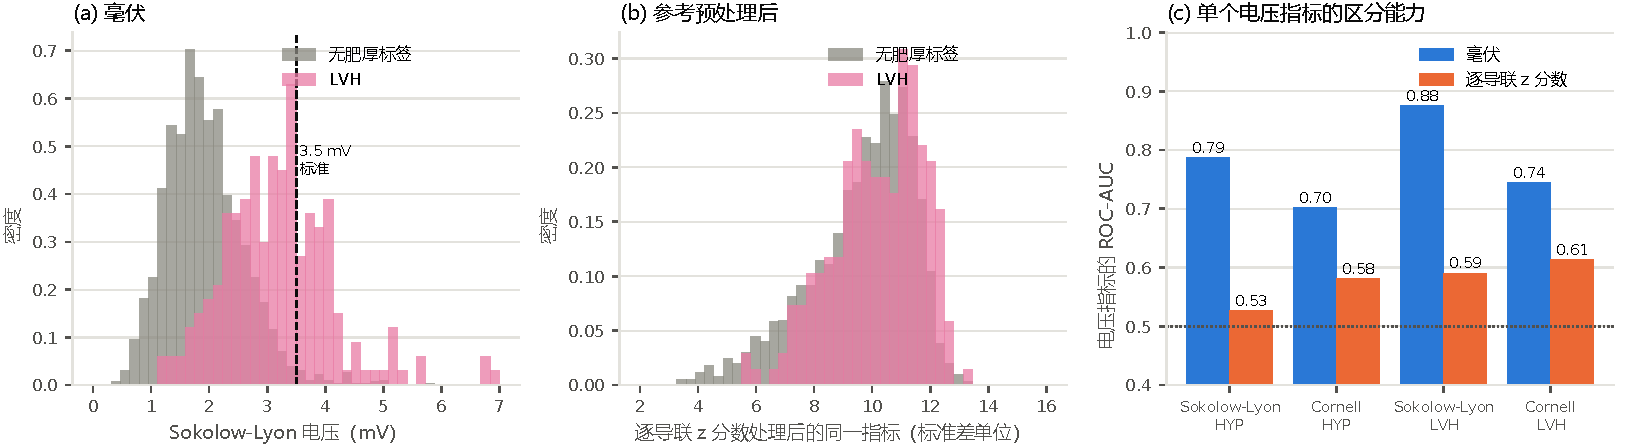
\includegraphics[width=\linewidth]{f03_voltage.pdf}
\caption{无需训练的电压信息探针。展示毫伏信号和逐导联标准化信号上的电压分布及判别结果。LVH 为左心室肥厚子类，HYP 为肥厚大类。分位数近似仅用于本研究的信息分析，不等同于临床人工测量。}
\label{fig:voltage}
\end{figure}

\subsection{幅值保留对 VOLT-KD 分类性能的贡献}\label{sec:input}
幅值保留在固定学生结构下带来主要分类收益，并在完整监督条件下保持有效（表\ref{tab:ladder}）。在使用相同子类与教师监督的 VOLT-KD 中，毫伏输入相对 z-score 输入将宏平均 ROC-AUC 从 0.9179 提高至 0.9298，宏平均 AP 从 0.7949 提高至 0.8274，宏平均 F1 从 0.7283 提高至 0.7542。HYP ROC-AUC 同时由 0.8414 提高至 0.8945。网络容量和监督目标保持一致时，三项整体指标及 HYP 判别共同改善，说明保留输入电压能够为已有知识学习提供更有效的信号基础。

仅使用五类硬标签训练时，毫伏输入已将 VOLT-KD 学生的宏平均 ROC-AUC 从 0.9106 提高至 0.9277，五种子配对差为 0.0171，95\% 区间为 [0.0142, 0.0201]；宏平均 F1 由 0.7189 提高至 0.7484。HYP ROC-AUC 的增量为 0.0734，从 0.8285 提高至 0.9019，占宏平均 AUC 增量的算术贡献约为 85.7\%。这一类别集中性与电压探针结果一致：恢复幅值相关线索对肥厚识别尤其有利。收益在引入子类和教师监督之前已经出现，确立了输入设计在完整框架中的基础作用。

两种监督条件下均出现输入收益（图\ref{fig:ladder}），表明幅值保留既服务于硬标签训练，也能与训练期知识学习共同使用。完整 VOLT-KD 获得较高的宏平均 AUC、AP 和 F1，而仅大类监督的毫伏学生具有更高的 HYP AUC。这种差异说明，整体决策质量与单类排序能力对监督的响应不同，输入收益与监督收益需要分别评价。

\begin{table}[htbp]
\centering\footnotesize
\setlength{\tabcolsep}{3pt}
\caption{VOLT-KD 学生的输入与监督消融。数值为五种子均值与标准差；完整监督包含大类硬标签、子类目标和 ECGFounder 教师软标签，粗体表示各列最高均值。}\label{tab:ladder}
\begin{tabularx}{\linewidth}{Yrrrr}
\toprule
配置 & 宏平均 AUC & HYP AUC & 宏平均 AP & 宏平均 F1 \\
\midrule
VOLT-KD 学生（仅大类，z-score） & $0.9106\pm0.0008$ & $0.8285\pm0.0044$ & $0.7795\pm0.0019$ & $0.7189\pm0.0039$ \\
VOLT-KD 学生（仅大类，毫伏） & $0.9277\pm0.0017$ & $\boldsymbol{0.9019\pm0.0026}$ & $0.8238\pm0.0029$ & $0.7484\pm0.0028$ \\
VOLT-KD 学生（大类+子类，毫伏） & $0.9280\pm0.0023$ & $0.9018\pm0.0033$ & $0.8240\pm0.0043$ & $0.7499\pm0.0022$ \\
\midrule
VOLT-KD 学生（完整监督，z-score） & $0.9179\pm0.0011$ & $0.8414\pm0.0039$ & $0.7949\pm0.0022$ & $0.7283\pm0.0022$ \\
VOLT-KD 学生（完整模型，毫伏） & $\boldsymbol{0.9298\pm0.0012}$ & $0.8945\pm0.0018$ & $\boldsymbol{0.8274\pm0.0020}$ & $\boldsymbol{0.7542\pm0.0009}$ \\
\bottomrule
\end{tabularx}
\par\vspace{3pt}{\footnotesize 各配置使用相同 VOLT-KD 骨干。“仅大类”配置仅使用五类硬标签，“大类+子类”配置增加子类目标，均不使用蒸馏。}
\end{table}
\begin{figure}[htbp]
\centering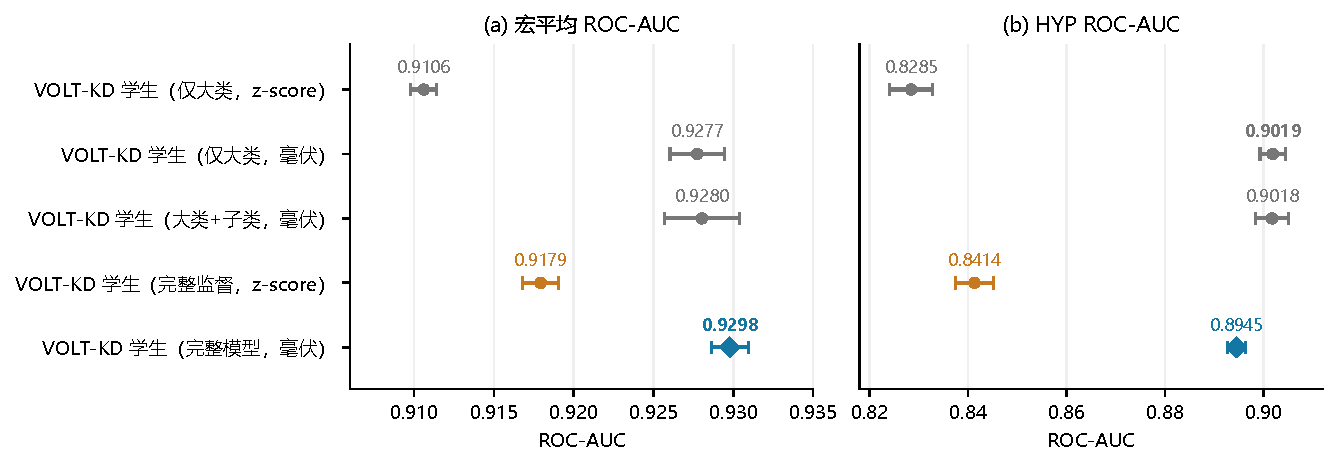
\includegraphics[width=\linewidth]{f11_ablation_ladder.pdf}
\caption{VOLT-KD 及输入、监督配置的宏平均与 HYP ROC-AUC。蓝色菱形为完整 VOLT-KD，橙色点为相同完整监督下的 z-score 对照，灰色点为仅大类或大类与子类监督的消融配置；误差线为五种子标准差。}
\label{fig:ladder}
\end{figure}

\subsection{跨骨干结果验证输入设计的可迁移性}
幅值保留的收益同时出现在循环学生骨干和状态空间骨干中（表\ref{tab:backbones}）。在 VOLT-KD 骨干上，仅大类监督和完整监督的宏平均 AUC 分别由 0.9106、0.9179 提高至 0.9277、0.9298。对于本地 MSCA-Mamba，保持网络与训练配方一致时，毫伏输入将宏平均 AUC 从 0.8950 提高至 0.9157，配对增量为 0.0207，95\% 区间为 [0.0188, 0.0227]。

本地 MSCA-Mamba 的 HYP ROC-AUC 从 0.8013 提高至 0.8879，约占宏平均 AUC 增量的 83.5\%，与 VOLT-KD 学生的类别收益分布相近。两种骨干采用不同的时序聚合方式，却均主要在幅值相关类别上获益，说明该改进具有输入层面的共性，而非依赖某一种序列模块。

MSCA-Mamba 的输入对照未采用 VOLT-KD 学生的噪声增强，仍获得一致的改善方向。结合完整监督下的输入对照，幅值保留在本文测试的两种紧凑骨干及不同监督条件下均有效。这使输入设计成为可复用的轻量化策略：通过提高已有参数所能利用的信息质量改善分类，而不依赖扩大模型容量。

\begin{table}[htbp]
\centering\small
\caption{VOLT-KD 与本地 MSCA-Mamba 的输入对照。数值为五种子宏平均 ROC-AUC 的均值与标准差；每行固定骨干、监督与训练设置，仅比较输入处理，粗体标记行内较高结果。}\label{tab:backbones}
\begin{tabularx}{\linewidth}{Yrr}
\toprule
骨干与监督 & z-score 输入 & 毫伏输入 \\
\midrule
VOLT-KD 骨干（五类硬标签） & $0.9106\pm0.0008$ & $\boldsymbol{0.9277\pm0.0017}$ \\
MSCA-Mamba 骨干（本文实现） & $0.8950\pm0.0024$ & $\boldsymbol{0.9157\pm0.0012}$ \\
\midrule
VOLT-KD 学生（完整模型） & $0.9179\pm0.0011$ & $\boldsymbol{0.9298\pm0.0012}$ \\
\bottomrule
\end{tabularx}
\par\vspace{3pt}{\footnotesize 完整 VOLT-KD 同时使用五大类硬标签、诊断子类目标和教师软标签；其两种输入配置采用相同监督。}
\end{table}

\subsection{训练期知识学习提升决策表现}\label{sec:supervision}
在有效的毫伏表征上增加训练监督，可以进一步改善学生的分类决策，而保持部署结构不变。表\ref{tab:effects}采用相同种子的配对差评价子类目标与 ECGFounder 教师监督的增量。

在已有大类与子类监督的 VOLT-KD 学生上加入蒸馏后，宏平均 F1 从 0.7499 提高至 0.7542，配对增量为 0.0043，95\% 区间为 [0.0022, 0.0064]。分类阈值由验证集确定，因此这一增量对应实际二元标签决策的改善。教师和子类辅助头在部署时均被移除，说明额外训练知识能够转化为固定学生网络的决策收益，而不增加推理分支。

子类监督和蒸馏的宏平均 AUC 配对增量分别为 0.0003 和 0.0017，区间均包含零；教师监督的优势更清楚地体现在 F1 上。与输入对照的较大 AUC 增量相比，这些结果表明，幅值保留主要改善诊断信息的可用性，软标签监督进一步调整验证阈值下的精确率与召回率权衡。子类目标提供了共享表征的细粒度约束，其独立排序收益在当前任务上较小。

教师知识的作用具有类别差异。ECGFounder 四教师集成的宏平均 AUC 为 0.9323，HYP AUC 为 0.8843；毫伏输入、含子类监督且无蒸馏的 VOLT-KD 学生在 HYP 上达到 0.9018，加入蒸馏后为 0.8945，配对变化为 $-0.0072$，95\% 区间为 [$-0.0099$, $-0.0045$]。整体 F1 改善与 HYP 排序下降并存，说明高总体性能教师的监督价值应结合目标类别评价。对 VOLT-KD 而言，学生自身的幅值表征已经为 HYP 提供较强判别能力，知识迁移的设计重点因而是保留这一优势，并利用教师改善整体决策。

样本内教师训练的 VOLT-KD 学生宏平均 AUC 为 0.9304，交叉拟合教师训练的学生为 0.9298。交叉拟合使每条训练记录的软标签来自未使用其微调折的教师，为监督目标提供明确的留出约束；样本内方案的分数略高。两套教师分别使用六折和八折微调数据，交叉拟合的作用在于约束目标生成过程，其精度效应还受到教师微调数据量的影响。
\begin{table}[htbp]
\centering\footnotesize
\setlength{\tabcolsep}{4pt}
\caption{本文 VOLT-KD 学生模型的配置配对比较。每项为前一配置减后一配置的五种子平均差及 95\% 区间；正值表示前者较高。区间反映训练随机性，未经多重比较校正。}\label{tab:effects}
\begin{tabularx}{\linewidth}{Yrrr}
\toprule
VOLT-KD 学生配置（前者 $-$ 后者） & 宏平均 AUC & HYP AUC & 宏平均 F1 \\
\midrule
VOLT-KD 学生（仅大类，毫伏） $-$ VOLT-KD 学生（仅大类，z-score） & \shortstack{$+0.0171$\\$[0.0142,\,0.0201]$} & \shortstack{$+0.0734$\\$[0.0682,\,0.0786]$} & \shortstack{$+0.0295$\\$[0.0249,\,0.0340]$} \\
VOLT-KD 学生（大类+子类，毫伏） $-$ VOLT-KD 学生（仅大类，毫伏） & \shortstack{$+0.0003$\\$[-0.0011,\,0.0017]$} & \shortstack{$-0.0002$\\$[-0.0058,\,0.0055]$} & \shortstack{$+0.0016$\\$[-0.0014,\,0.0045]$} \\
VOLT-KD 学生（完整模型） $-$ VOLT-KD 学生（大类+子类，无蒸馏） & \shortstack{$+0.0017$\\$[-0.0003,\,0.0038]$} & \shortstack{$-0.0072$\\$[-0.0099,\,-0.0045]$} & \shortstack{$+0.0043$\\$[0.0022,\,0.0064]$} \\
VOLT-KD 学生（交叉拟合教师） $-$ VOLT-KD 学生（样本内教师） & \shortstack{$-0.0006$\\$[-0.0012,\,-0.0001]$} & \shortstack{$-0.0056$\\$[-0.0080,\,-0.0031]$} & \shortstack{$-0.0018$\\$[-0.0079,\,0.0043]$} \\
\bottomrule
\end{tabularx}
\par\vspace{3pt}{\footnotesize 除输入处理对照外，各配置均使用毫伏输入。无蒸馏配置使用大类与子类目标；教师方案对照比较相应软标签训练所得的 VOLT-KD 学生。}

\end{table}


训练期知识学习使高容量教师能够服务于低容量部署模型（表\ref{tab:teacher}和图\ref{fig:teacher}）。单个 ECGFounder 教师包含 30,693,964 个参数，四教师集成共 122,775,856 个参数；VOLT-KD 部署学生仅有 107,189 个参数，分别为单教师和四教师总参数量的约 $1/286.4$ 与 $1/1145.4$，减少 99.65\% 和 99.91\%。教师规模与部署规模由此分离，额外知识无需通过保留高容量推理网络来使用。

在这一参数规模下，VOLT-KD 的宏平均 AUC 和 AP 与四教师集成仅相差 0.0025 和 0.0031，宏平均 F1 则由教师的 0.7482 提高至 0.7542，HYP AUC 由 0.8843 提高至 0.8945。相较八折单教师，学生的宏平均 AUC 仅低 0.0005，AP 和 F1 分别高出 0.0025 和 0.0086。小规模学生由此保留了接近教师的整体排序能力，并取得更高的阈值分类 F1。结合无蒸馏学生已经较高的 AUC，这一性能与规模权衡来自幅值输入、紧凑表征及训练监督的共同设计，其中蒸馏的可量化增量主要体现在最终分类决策。

\begin{table}[htbp]
\centering\footnotesize
\setlength{\tabcolsep}{3pt}
\caption{ECGFounder 教师与本文 VOLT-KD 学生的性能及模型规模比较。ECGFounder\cite{li2025} 的测试值来自本项目微调评价；教师结果来自一组评价，学生为五种子均值。参数量按部署配置统计，M 表示百万；性能指标越高越好，参数量越低越好，最优值加粗。}\label{tab:teacher}
\begin{tabularx}{\linewidth}{Ycrrrrr}
\toprule
配置 & 输入 & \shortstack{参数量\\（M）} & \shortstack{宏平均\\AUC} & \shortstack{宏平均\\AP} & \shortstack{宏平均\\F1} & HYP AUC \\
\midrule
ECGFounder 四教师集成 & 500 Hz & 122.7759 & \textbf{0.9323} & \textbf{0.8305} & 0.7482 & 0.8843 \\
ECGFounder 八折单教师 & 500 Hz & 30.6940 & 0.9303 & 0.8249 & 0.7456 & 0.8795 \\
VOLT-KD 学生（无蒸馏） & 100 Hz & \textbf{0.1072} & $0.9280\pm0.0023$ & 0.8240 & 0.7499 & \textbf{0.9018} \\
VOLT-KD 学生（样本内教师） & 100 Hz & \textbf{0.1072} & $0.9304\pm0.0011$ & 0.8282 & \textbf{0.7560} & 0.9001 \\
VOLT-KD & 100 Hz & \textbf{0.1072} & $0.9298\pm0.0012$ & 0.8274 & 0.7542 & 0.8945 \\
\bottomrule
\end{tabularx}
\par\vspace{3pt}{\footnotesize 四教师集成按四个独立模型的参数总和计数，测试集结果由四个模型的 logits 平均后评价；训练记录的软标签分别来自相应留出教师。各学生配置共享同一部署结构，均移除训练用辅助头；参数倍数由未舍入的参数总数计算。}
\end{table}

\begin{figure}[htbp]
\centering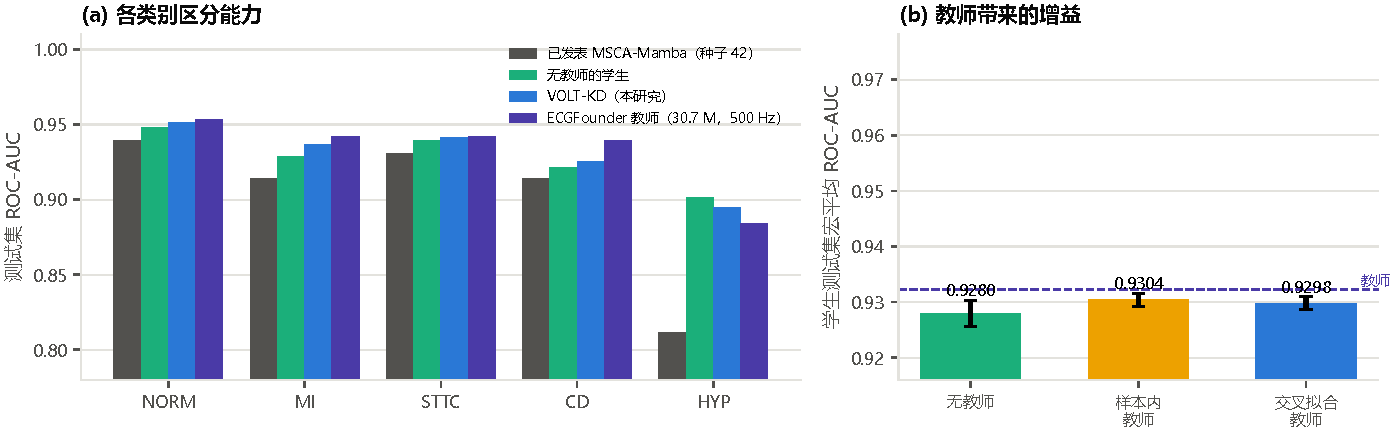
\includegraphics[width=\linewidth,height=0.38\textheight,keepaspectratio]{f24_teacher_student.pdf}
\caption{ECGFounder 教师与本文 VOLT-KD 学生的逐类及整体结果。教师为四个留出模型的测试集 logits 集成；学生为五种子均值；图内教师参数量按单个成员标注，集成总参数量见表\ref{tab:teacher}；文献 MSCA-Mamba 为原文种子 42 参照。}\label{fig:teacher}
\end{figure}


\subsection{逐类与诊断子类结果定位性能改善}
完整 VOLT-KD 的改善兼顾整体分类和幅值相关诊断（图\ref{fig:perclass}）。NORM、MI、STTC 和 CD 的五种子 ROC-AUC 分别为 0.9511、0.9365、0.9417 和 0.9251，HYP ROC-AUC 为 0.8945，AP 为 0.650。多种类别在同一紧凑骨干上获得有效区分，说明毫伏输入能够与形态及时序表征共同使用。HYP 的较低 AP 同时反映了该类在低阳性比例条件下更困难的精确率—召回率权衡，因而需要结合逐类结果评价幅值设计。
\begin{figure}[htbp]
\centering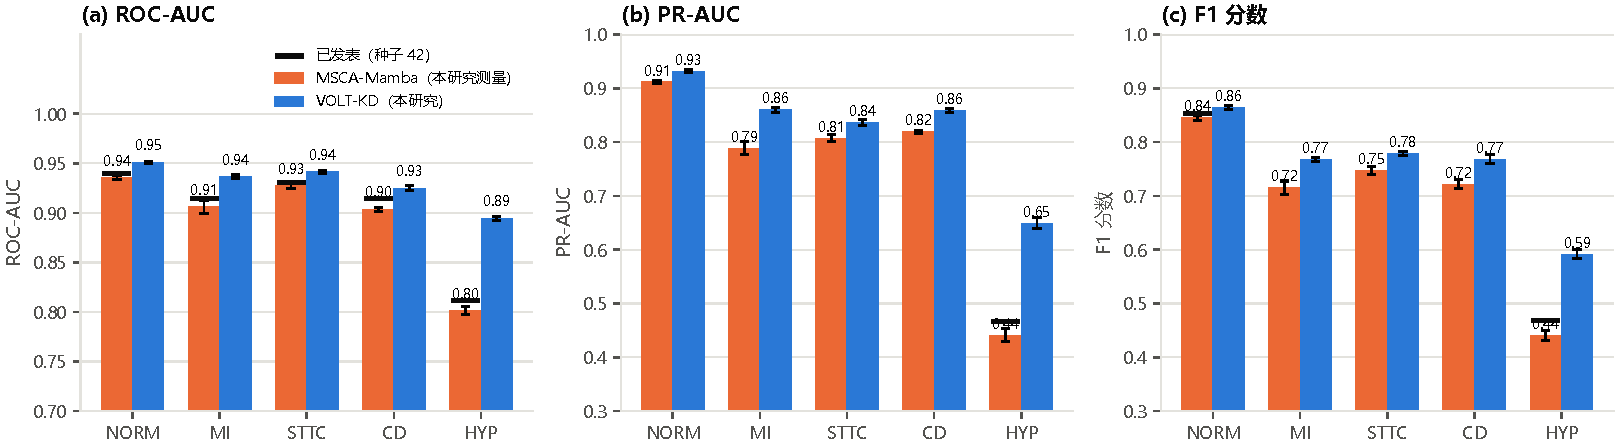
\includegraphics[width=\linewidth,height=0.38\textheight,keepaspectratio]{f07_per_class.pdf}
\caption{完整 VOLT-KD 与本地 MSCA-Mamba 的逐类 ROC-AUC、PR-AUC/AP 和 F1。柱形及误差线为五种子均值与标准差；黑色横线为 MSCA-Mamba 文献的种子 42 结果\cite{cetintas2026}。}\label{fig:perclass}
\end{figure}

在种子 42 的对应比较中，VOLT-KD 的 HYP ROC-AUC、AP 和 F1 分别为 0.8930、0.6607 和 0.6035，高于 MSCA-Mamba 文献报告的 0.8115、0.4662 和 0.4682；召回率由 0.4924 提高至 0.6565。五种子完整 VOLT-KD 的 HYP 召回率为 0.6191、特异度为 0.9347（表\ref{tab:class}）。因此，幅值相关类别的排序改善还伴随更多阳性记录被检出，并非仅表现为分数排序变化。文献比较与固定骨干输入对照在 HYP 上的同向结果，加强了幅值信息与肥厚识别收益之间的联系。

诊断子类评价进一步定位了幅值设计的受益对象（图\ref{fig:subclass}和表\ref{tab:subclass}）。在携带 LVH 子类标签的记录中，完整 VOLT-KD 将父类 HYP 判为阳性的比例为 0.721，本地 MSCA-Mamba 为 0.595；IRBBB 和 AVB 的父类检出比例分别增加约 9.1 和 11.7 个百分点，AMI 与 IMI 也有所改善。LVH 的提高与电压探针及 HYP 输入对照相吻合，使整体增益落实到具有电压依据的具体诊断子类。IVCD 的对应比例由 0.327 降至 0.289，说明共享骨干对不同诊断形态的收益仍有差异。
\begin{figure}[htbp]
\centering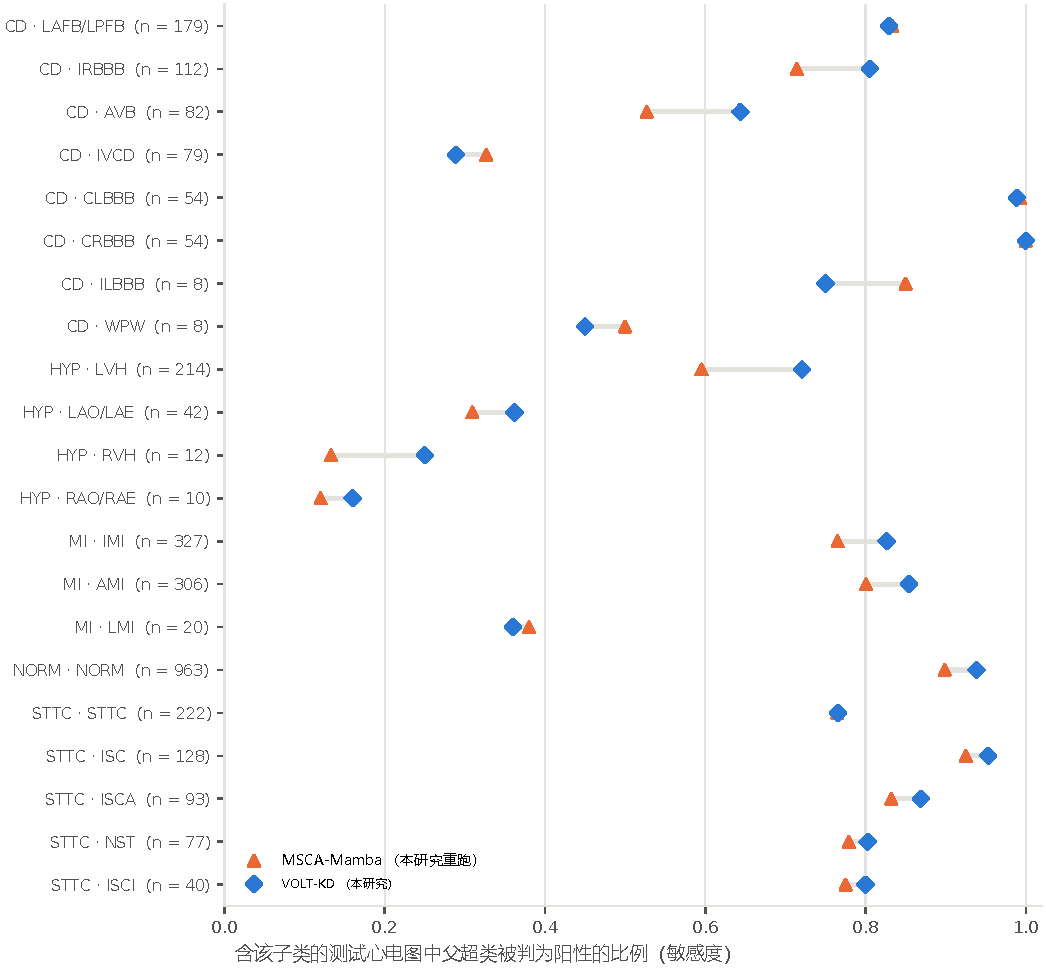
\includegraphics[width=\linewidth,height=0.58\textheight,keepaspectratio]{f16_subclass_sensitivity.pdf}
\caption{完整 VOLT-KD 与本地 MSCA-Mamba 在各诊断子类记录中的父类检出比例。纳入至少五条测试记录的子类，数值和样本量见表\ref{tab:subclass}。}\label{fig:subclass}
\end{figure}

\subsection{VOLT-KD 的组件消融与学生结构简化}
以完整 VOLT-KD 为参照，输入替换、监督移除和结构简化呈现不同的性能影响（表\ref{tab:loo}和图\ref{fig:loo}）。这些变体分别改变 z-score 输入、子类损失、教师生成方案、分类头、GRU 层或网络宽度，其余设置沿用对应完整配置。该对照将信息保留的作用与网络容量及监督目标的作用分开评价。

完整 VOLT-KD 改用 z-score 后，宏平均 AUC 由 0.9298 降至 0.9179，HYP AUC 由 0.8945 降至 0.8414。即使保留子类和教师监督，移除毫伏表示仍造成明显下降，表明丰富的训练目标并未替代输入尺度所承载的信息。与仅大类监督下的输入收益结合，幅值保留在学习早期和完整知识学习流程中均构成有效基础。
\begin{table}[htbp]
\centering\footnotesize
\setlength{\tabcolsep}{3pt}
\caption{完整 VOLT-KD 及其组件消融、结构简化变体。数值为表列种子数下的均值与标准差，参数量按训练阶段统计。}\label{tab:loo}
\begin{tabularx}{\linewidth}{Yrrrrr}
\toprule
VOLT-KD 学生配置 & 种子数 & 训练参数量 & 宏平均 AUC & 宏平均 F1 & HYP AUC \\
\midrule
VOLT-KD（完整模型，毫伏输入） & 5 & 112,364 & $0.9298\pm0.0012$ & $0.7542\pm0.0009$ & $0.8945\pm0.0018$ \\
VOLT-KD 学生（z-score 输入） & 5 & 112,364 & $0.9179\pm0.0011$ & $0.7283\pm0.0022$ & $0.8414\pm0.0039$ \\
VOLT-KD 学生（无子类监督） & 5 & 112,364 & $0.9299\pm0.0007$ & $0.7519\pm0.0031$ & $0.8943\pm0.0009$ \\
VOLT-KD 学生（样本内教师） & 5 & 112,364 & $0.9304\pm0.0011$ & $0.7560\pm0.0047$ & $\boldsymbol{0.9001\pm0.0034}$ \\
VOLT-KD 学生（noisy-OR 分类头） & 3 & 111,239 & $\boldsymbol{0.9310\pm0.0004}$ & $0.7537\pm0.0023$ & $0.8970\pm0.0012$ \\
VOLT-KD 学生（无 GRU 层） & 3 & 59,692 & $0.9303\pm0.0003$ & $0.7541\pm0.0012$ & $0.8934\pm0.0031$ \\
VOLT-KD 学生（宽度减半） & 3 & \textbf{56,444} & $0.9298\pm0.0018$ & $\boldsymbol{0.7585\pm0.0029}$ & $0.8935\pm0.0024$ \\
\bottomrule
\end{tabularx}
\par\vspace{3pt}{\footnotesize 除 z-score 变体外，各 VOLT-KD 学生均使用毫伏输入。无子类监督变体关闭子类硬标签与蒸馏损失，保留辅助头结构，因此训练参数量不变。完整 VOLT-KD 的训练参数量为 112,364；表\ref{tab:teacher}的 107,189 为移除辅助头后的部署参数量。}

\end{table}

关闭子类监督后，VOLT-KD 的宏平均 AUC 为 0.9299，接近完整模型的 0.9298，F1 则由 0.7542 降至 0.7519。子类目标的作用因而更多体现在分类决策，而非整体排序。宽度减半和移除 GRU 的学生分别使用 56,444 和 59,692 个训练参数，宏平均 AUC 仍达到 0.9298 和 0.9303。三种子变体与完整模型的共同种子配对结果显示，精简后的网络仍能利用毫伏输入形成有效表征。对轻量化而言，这说明幅值保留的价值不依赖完整 GRU 或较宽通道，也为进一步压缩部署网络提供了实验证据。
\begin{figure}[htbp]
\centering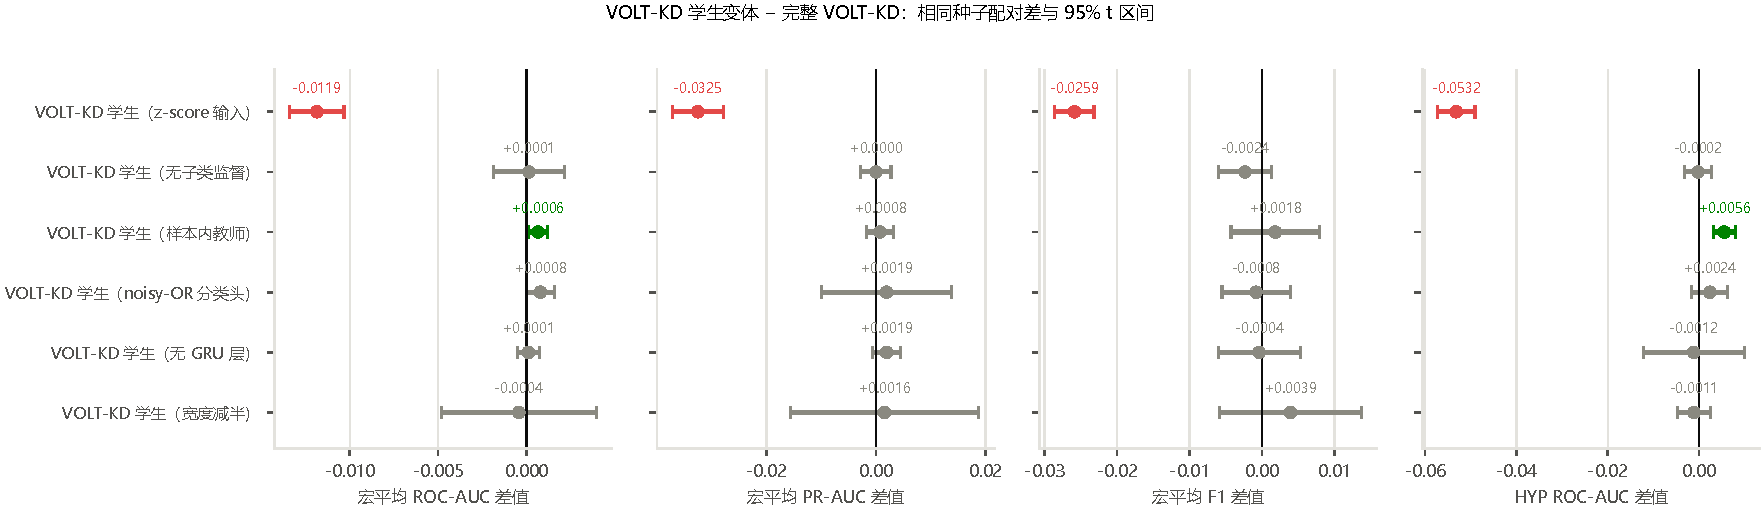
\includegraphics[width=\linewidth,height=0.45\textheight,keepaspectratio]{f12_ablation_leave_one_out.pdf}
\caption{本文 VOLT-KD 各变体相对完整 VOLT-KD 的指标差。差值方向为学生变体减完整 VOLT-KD；点和区间采用相同种子的配对差及 95\% $t$ 区间，主要变体设置见表\ref{tab:loo}。}\label{fig:loo}
\end{figure}


\subsection{增益响应与导联分析解释模型利用的信息}
VOLT-KD 的 HYP 决策随输入电压增益系统变化（图\ref{fig:gain}）。对同一测试记录分别施加 0.5、1 和 2 倍增益时，完整 VOLT-KD 预测 HYP 阳性的比例约为 2.0\%、13.3\% 和 52.3\%，逐导联标准化的本地 MSCA-Mamba 维持在约 16.6\%。VOLT-KD 对幅值变化的响应表明，保留的电压尺度实际参与了预测，而非仅作为未被利用的输入信息。

电压探针揭示幅值与肥厚标签的对应，固定骨干对照显示保留该信息的分类收益，增益干预则确认模型输出对该信息的响应。三类证据共同支持 VOLT-KD 将物理电压纳入轻量表征的设计。增益敏感性也意味着采集单位和设备校准直接关系到输出一致性：保留诊断幅值的同时，需要维持训练与使用阶段的毫伏换算一致。
\begin{figure}[htbp]
\centering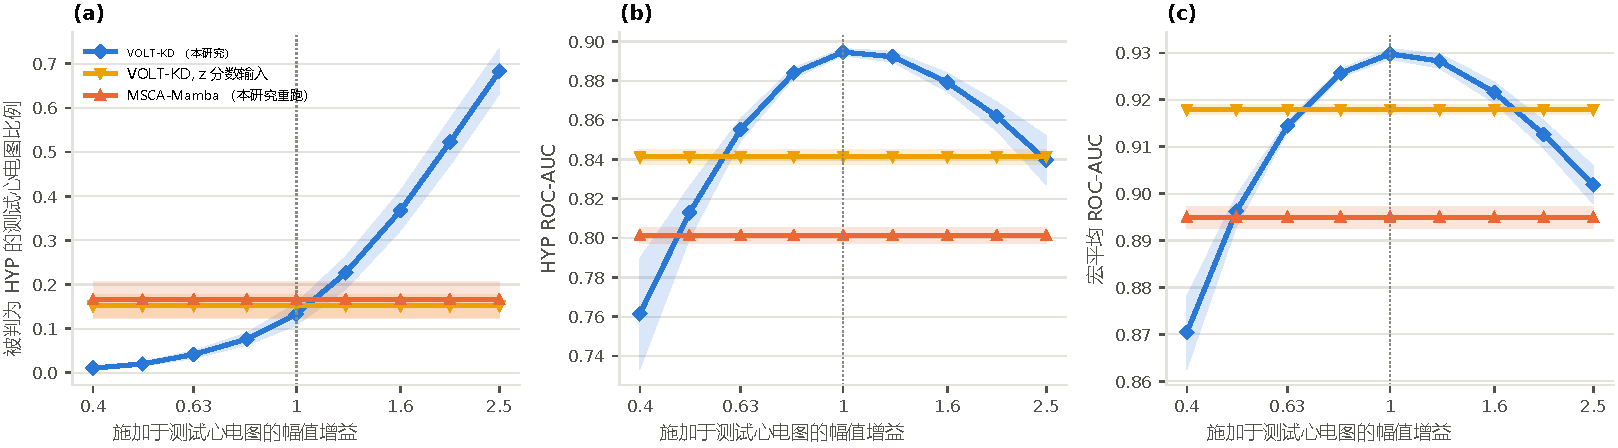
\includegraphics[width=\linewidth]{f13_gain_probe.pdf}
\caption{完整 VOLT-KD、其 z-score 输入对照与本地 MSCA-Mamba 对全局电压增益的响应。相同测试波形乘以给定增益，模型参数、标签及验证阈值保持固定。}
\label{fig:gain}
\end{figure}

导联配置改变了紧凑学生能够利用的空间观测信息。表\ref{tab:leads}比较完整十二导联 VOLT-KD、六肢体导联学生和仅 II 导联学生；各配置分别训练，共享骨干、毫伏预处理及大类、子类和十二导联教师监督。保持十二通道接口并将未用通道置零，使该实验在相同网络容量下评价导联信息的作用。

六肢体导联 VOLT-KD 的宏平均 AUC 为 $0.8964\pm0.0015$，较仅 II 导联的 $0.8566\pm0.0010$ 高出 0.0398；HYP AUC 分别为 0.8476 和 0.7901。网络规模相同时，增加肢体导联带来的改善说明，多方向电活动观测能为有限容量的学生补充有效信息。完整十二导联模型在四项指标上均取得最高均值，进一步表明幅值信息的价值与导联覆盖共同决定分类能力。VOLT-KD 的统一骨干和训练目标可用于不同采集配置，其轻量化优势来自紧凑计算结构，而保留更多导联有助于减少信息损失。

\begin{table}[htbp]
\centering\footnotesize
\setlength{\tabcolsep}{3pt}
\caption{完整十二导联 VOLT-KD 与分别训练的六肢体导联、单 II 导联学生的分类性能。数值为表列种子数下的均值与标准差，粗体表示各列最高均值。}\label{tab:leads}
\begin{tabularx}{\linewidth}{Yrrrrr}
\toprule
VOLT-KD 学生配置 & 种子数 & 宏平均 AUC & 宏平均 AP & 宏平均 F1 & HYP AUC \\
\midrule
VOLT-KD（十二导联） & 5 & $\boldsymbol{0.9298\pm0.0012}$ & $\boldsymbol{0.8274\pm0.0020}$ & $\boldsymbol{0.7542\pm0.0009}$ & $\boldsymbol{0.8945\pm0.0018}$ \\
VOLT-KD 学生（六肢体导联） & 3 & $0.8964\pm0.0015$ & $0.7597\pm0.0036$ & $0.6922\pm0.0062$ & $0.8476\pm0.0003$ \\
VOLT-KD 学生（仅 II 导联） & 3 & $0.8566\pm0.0010$ & $0.6828\pm0.0012$ & $0.6367\pm0.0008$ & $0.7901\pm0.0018$ \\
\bottomrule
\end{tabularx}
\par\vspace{3pt}{\footnotesize 各 VOLT-KD 学生采用十二导联 ECGFounder 软标签训练。学生结构与监督设置相同，保持十二通道接口并将未使用的通道置零。六肢体导联为 I、II、III、aVR、aVL 和 aVF；单导联变体仅保留 II 导联。}

\end{table}
\subsection{VOLT-KD 与 MSCA-Mamba 的测试亚组比较}
完整 VOLT-KD 相对本地 MSCA-Mamba 的优势在多个测试亚组中保持一致（图\ref{fig:subgroups}和表\ref{tab:subgroup}）。两种模型使用固定训练权重，在同一 PTB-XL 测试折按性别、年龄、设备、质量与标签共现分组评价，以检验总体收益是否集中于少数记录条件。

在男性和女性组中，完整 VOLT-KD 的宏平均 AUC 分别为 0.940 和 0.920，本地 MSCA-Mamba 为 0.906 和 0.884。四个年龄组均有改善，75 岁及以上组的 AUC 由本地 MSCA-Mamba 的 0.859 提高至 VOLT-KD 的 0.906；四种主要设备分组的增量约为 0.038--0.040。增益分布于不同人群和设备条件，说明完整输入与学习流程的总体优势具有较广的内部覆盖，而非由某个高分亚组主导。

在有噪声标记的 513 条记录中，完整 VOLT-KD 的宏平均 AUC 为 0.923，本地 MSCA-Mamba 为 0.887；在携带多个大类标签的 508 条记录中，两者分别为 0.896 和 0.852。自然质量问题及异常共存条件下仍有收益，支持紧凑表征同时处理受干扰形态和多标签线索。该结果扩展了受控输入实验的观察条件，评价的是完整 VOLT-KD 的组内适应性。不同亚组的绝对分数仍有差异，当前证据范围为 PTB-XL 内部人群与设备分布。
\begin{figure}[htbp]
\centering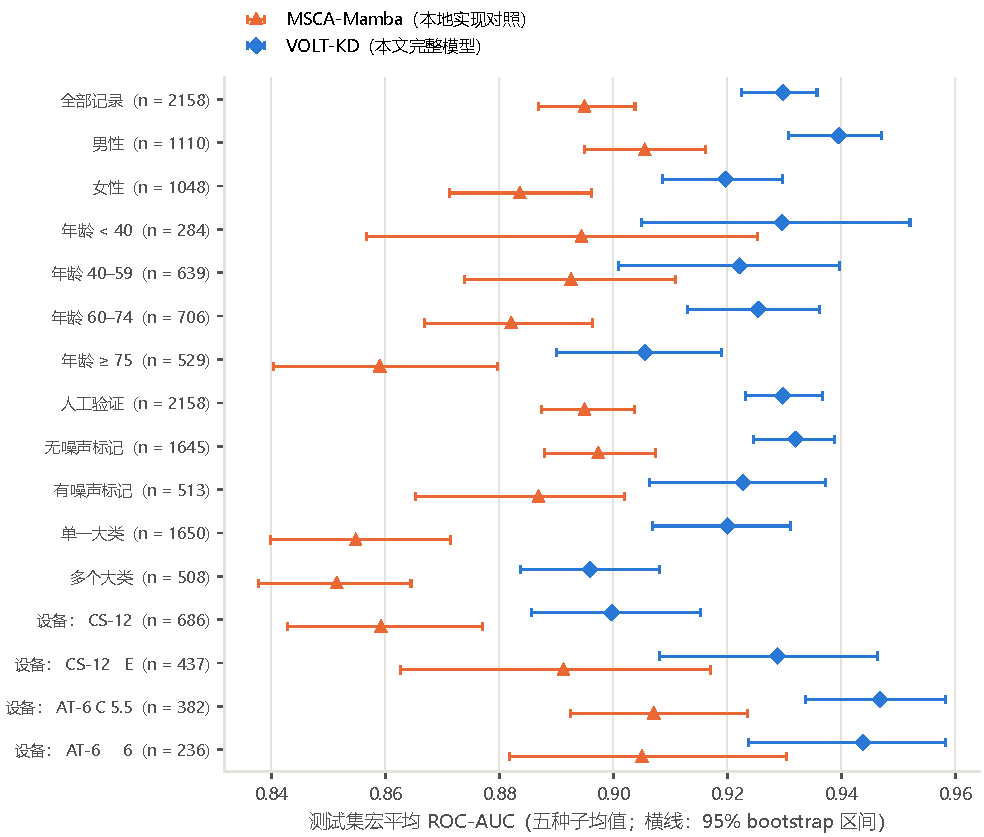
\includegraphics[width=\linewidth,height=0.57\textheight,keepaspectratio]{f17_subgroups.pdf}
\caption{本文完整 VOLT-KD 学生模型与本地 MSCA-Mamba 对照模型在不同测试亚组中的宏平均 ROC-AUC。蓝色菱形为完整 VOLT-KD，橙色三角形为 MSCA-Mamba 本地实现；点表示各模型五个种子的指标均值，横向区间为各组内 300 次记录级 bootstrap 得到的 95\% 区间。两种模型在同一测试折按人口、设备、质量和标签共现条件分组评价；具体样本量和数值见表\ref{tab:subgroup}。}\label{fig:subgroups}
\end{figure}

\subsection{概率质量与阈值决策分析}
VOLT-KD 的分类收益延伸至概率预测误差（表\ref{tab:calib}和图\ref{fig:calib}）。与本地 MSCA-Mamba 相比，完整 VOLT-KD 的平均 Brier 分数由 0.096 降至 0.081，五个类别均有下降，其中 HYP 由 0.088 降至 0.067。预测概率与标签之间的平方偏差减小，说明紧凑模型的性能改善并非只体现在排序，还体现在概率输出的整体质量。两模型平均 ECE 均约为 0.037，且 MI、CD、HYP 与 NORM、STTC 的变化方向不同；因此，概率误差降低与各类校准改善应分别评价。
\begin{table}[htbp]
\centering\footnotesize
\caption{完整 VOLT-KD 与本地 MSCA-Mamba 的逐类概率误差。数值为五种子均值与标准差；ECE 与 Brier 均越低越好。}\label{tab:calib}
\begin{tabularx}{\linewidth}{Yrrrr}
\toprule
类别 & 对照 ECE & VOLT-KD ECE & 对照 Brier & VOLT-KD Brier \\
\midrule
NORM & $\boldsymbol{0.057\pm0.007}$ & $0.065\pm0.005$ & $0.106\pm0.002$ & $\boldsymbol{0.096\pm0.001}$ \\
MI & $0.039\pm0.005$ & $\boldsymbol{0.036\pm0.007}$ & $0.105\pm0.003$ & $\boldsymbol{0.086\pm0.002}$ \\
STTC & $\boldsymbol{0.022\pm0.002}$ & $0.027\pm0.004$ & $0.089\pm0.002$ & $\boldsymbol{0.079\pm0.002}$ \\
CD & $0.040\pm0.007$ & $\boldsymbol{0.034\pm0.001}$ & $0.091\pm0.001$ & $\boldsymbol{0.076\pm0.001}$ \\
HYP & $0.029\pm0.005$ & $\boldsymbol{0.022\pm0.005}$ & $0.088\pm0.001$ & $\boldsymbol{0.067\pm0.001}$ \\
\bottomrule
\end{tabularx}
\par\vspace{3pt}{\footnotesize ECE 使用十个等宽概率区间。}
\end{table}

\begin{figure}[htbp]
\centering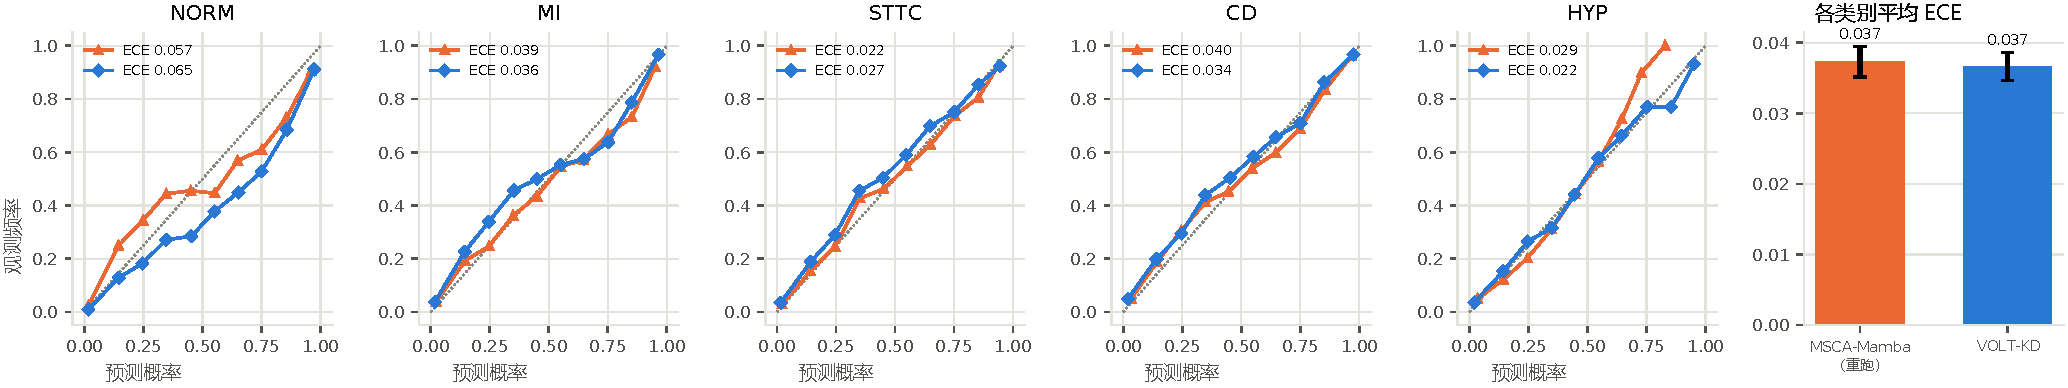
\includegraphics[width=\linewidth,height=0.50\textheight,keepaspectratio]{f19_calibration.pdf}
\caption{完整 VOLT-KD 与本地 MSCA-Mamba 的逐类可靠性曲线及 ECE。可靠性曲线比较预测概率与观察阳性频率。}\label{fig:calib}
\end{figure}

决策曲线将性能差异扩展到不同误报代价下的阈值选择（图\ref{fig:dca}）。净获益按 $\mathrm{NB}(t)=\mathrm{TP}/N-\mathrm{FP}/N\cdot t/(1-t)$ 计算。在 0.02--0.80、步长为 0.02 的阈值网格上，五类共 200 个“类别—阈值”组合中，VOLT-KD 有 195 个组合达到不低于本地 MSCA-Mamba 的净获益，占 97.5\%。这种跨阈值的一致性说明，完整方法的收益能够在多种误报权重下转化为分类决策优势，而不依赖单一操作点。该分析以数据库诊断标签为结局，支持的是算法层面的阈值决策表现。
\begin{figure}[htbp]
\centering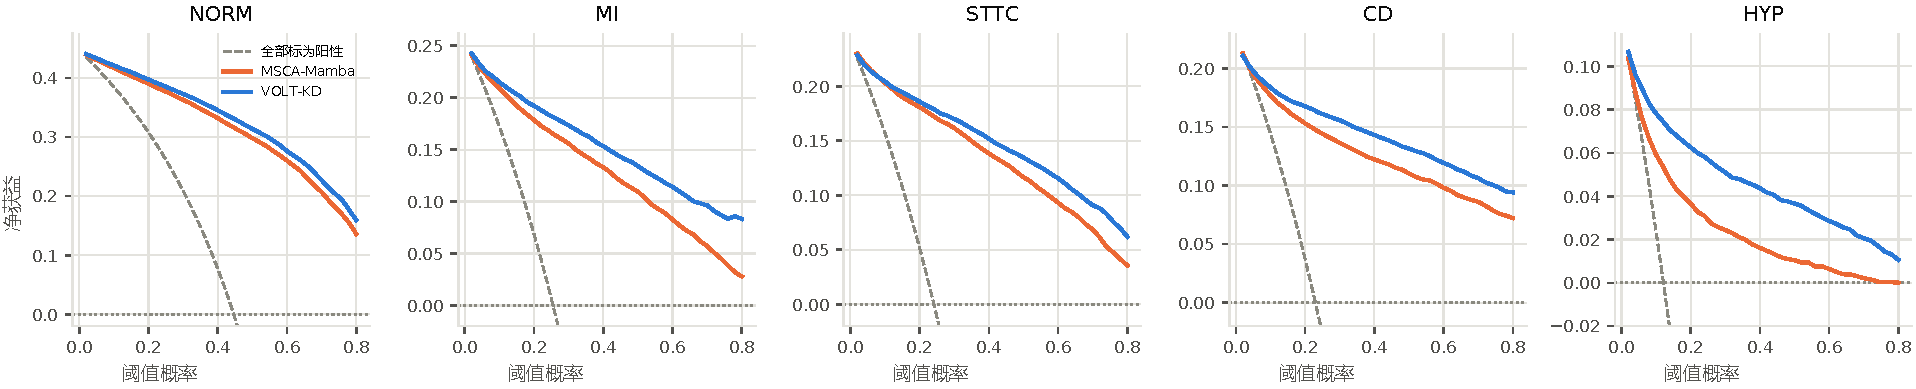
\includegraphics[width=\linewidth,height=0.40\textheight,keepaspectratio]{f20_decision_curves.pdf}
\caption{完整 VOLT-KD 与本地 MSCA-Mamba 的五类别决策曲线。净获益为五种子均值；参考线对应全部判为阳性与全部判为阴性，NORM 的阳性事件为正常标签。}\label{fig:dca}
\end{figure}

\subsection{VOLT-KD 与 MSCA-Mamba 的输入扰动对照}
幅值保留增加了输入尺度的可用性，其性能价值还取决于噪声条件下的稳定性。图\ref{fig:noise}在固定训练权重下比较完整 VOLT-KD 与本地 MSCA-Mamba，对相同测试记录分别施加基线漂移、高斯噪声和随机导联置零。扰动先作用于物理信号，再进入各模型原有的预处理与推理流程，从而评价完整分类流程对输入质量下降的响应。

基线漂移幅值为 0--2 mV，高斯噪声标准差为 0--0.2 mV，随机置零导联数为 0--8，各包含六个测试强度（表\ref{tab:noise_full}）。随机导联置零直接作用于十二导联训练模型，检验突发通道缺失；针对指定导联集合重新训练的结果见表\ref{tab:leads}。

在 0.5 mV 基线漂移下，完整 VOLT-KD 的宏平均 AUC 为 0.9058，本地 MSCA-Mamba 为 0.7309；相对于各自无扰动结果，下降幅度分别约为 0.0240 和 0.1641。高斯噪声标准差为 0.1 mV 时，两者分别为 0.9236 和 0.8499；随机置零四个导联时分别为 0.8823 和 0.8315。完整 VOLT-KD 在全部已测试强度上保持更高的 AUC，说明其性能优势延伸至渐进增强的信号干扰和观测缺失。幅值输入与紧凑特征提取、训练增强组合后，仍能在这些条件下保留较有效的诊断线索。随着强干扰或导联缺失增加，性能持续下降，表明物理信息保留与信号质量控制需要共同考虑。
\begin{figure}[htbp]
\centering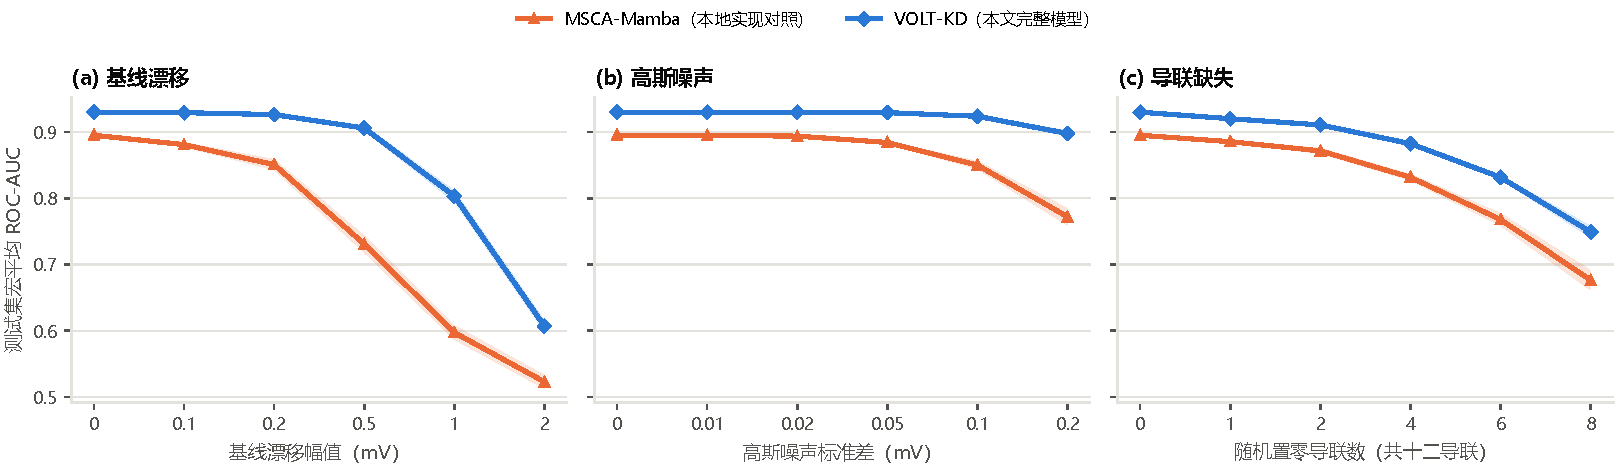
\includegraphics[width=\linewidth,height=0.43\textheight,keepaspectratio]{f18_noise_robustness.pdf}
\caption{本文完整 VOLT-KD 学生模型与本地 MSCA-Mamba 对照模型在测试输入受扰动时的宏平均 ROC-AUC。蓝色菱形为完整 VOLT-KD，橙色三角形为本地 MSCA-Mamba；点为五种子均值，阴影为 $\pm1$ 个标准差。(a) 低频基线漂移；(b) 高斯噪声；(c) 随机导联置零。零强度对应原始测试输入，模型参数固定；完整 AUC 数值见表\ref{tab:noise_full}。}\label{fig:noise}
\end{figure}


\subsection{紧凑设计的计算收益}
VOLT-KD 的信息利用收益伴随着较低的计算开销（表\ref{tab:efficiency}）。相较本地 MSCA-Mamba，学生部署参数减少 11.5\%，估计运算量减少 81.6\%，FP32 权重占用为 0.409 MiB。运算量降幅大于参数量降幅，与骨干对长序列计算的压缩一致：多尺度深度卷积降低时间滤波成本，共享逐点投影控制通道混合开销，两次下采样将 GRU 输入长度缩短为原来的四分之一。因而，轻量化收益不仅来自权重存储，也来自对计算发生位置和序列长度的组织。

在同一 NVIDIA GB10 平台上，VOLT-KD 的批量 256 吞吐率为每秒 10,397 条记录，本地 MSCA-Mamba 为 3,199 条，前者为后者的 3.25 倍。其单线程 CPU 推理延迟为 32.5 ms，约为十秒输入时长的 0.33\%。这些测量说明，较低的运算量能够转化为批量处理能力，并提供 CPU 推理路径。单条 GPU 延迟为 1.68 ms，高于对照的 1.26 ms；峰值 GPU 内存为 17.9 MiB，对照为 5.8 MiB。因此，当前结构的实测优势主要是批量吞吐与参数存储，具体运行配置仍需结合延迟和内存需求选择。

以 107,189 个部署参数达到宏平均 AUC 0.9298，表明幅值输入和训练期知识学习所带来的收益无需依赖高容量推理网络。参数、运算量与吞吐结果共同支持 VOLT-KD 的资源设计：训练时利用丰富监督，推理时以单一紧凑通路处理保留物理尺度的信号。
\begin{table}[htbp]
\centering\footnotesize
\caption{同一 NVIDIA GB10 平台上的八种结构计算特征。本文学生删除辅助头；所有参数与计算量来自本地实现。}\label{tab:efficiency}
\begin{tabularx}{\linewidth}{Yrrrrrr}
\toprule
模型 & 参数 & MFLOPs & \shortstack{GPU 延迟\\ms} & \shortstack{批量吞吐\\条/秒} & \shortstack{GPU 内存\\MiB} & \shortstack{CPU 延迟\\ms} \\
\midrule
VOLT-KD & 107,189 & \textbf{30.1} & 1.68 & 10,397 & 17.9 & 32.5 \\
MSCA-Mamba & 121,149 & 163.7 & 1.26 & 3,199 & 5.8 & -- \\
BiMamba & 214,077 & 292.7 & 1.66 & 1,788 & 6.6 & -- \\
匹配 Conv1D & 120,435 & 169.0 & 1.05 & 7,506 & 2.4 & 6.0 \\
匹配 GRU & 120,906 & 53.6 & 2.68 & 4,663 & 16.2 & 81.8 \\
匹配 LSTM & 120,953 & 50.6 & 2.78 & 4,930 & 16.7 & 41.0 \\
匹配 Transformer & 121,405 & 34.6 & 1.60 & 2,702 & 3.7 & 27.2 \\
多尺度 CNN & \textbf{51,141} & 34.6 & \textbf{0.54} & \textbf{17,066} & \textbf{1.5} & \textbf{1.9} \\
\bottomrule
\end{tabularx}
\par\vspace{3pt}{\footnotesize GPU 延迟为批量 1，吞吐为批量 256，CPU 为单线程。参数匹配控制及 BiMamba 的计时使用未训练权重，评价的是结构计算开销；MSCA-Mamba 与学生使用训练权重。-- 表示该实现未提供 CPU 计时。}
\end{table}


在八种本地结构中，VOLT-KD 的 30.1 MFLOPs 最低，批量吞吐高于匹配 Conv1D、GRU、LSTM、Transformer 和两种 Mamba 配置；更小的多尺度 CNN 具有更高吞吐（图\ref{fig:efficiency}）。这些差异表明，轻量网络的参数量、算术运算和实测速度分别受结构组织影响。VOLT-KD 的贡献在于获得较高分类性能与低运算量的组合，而非在所有资源指标上取同一最优值。
\begin{figure}[htbp]
\centering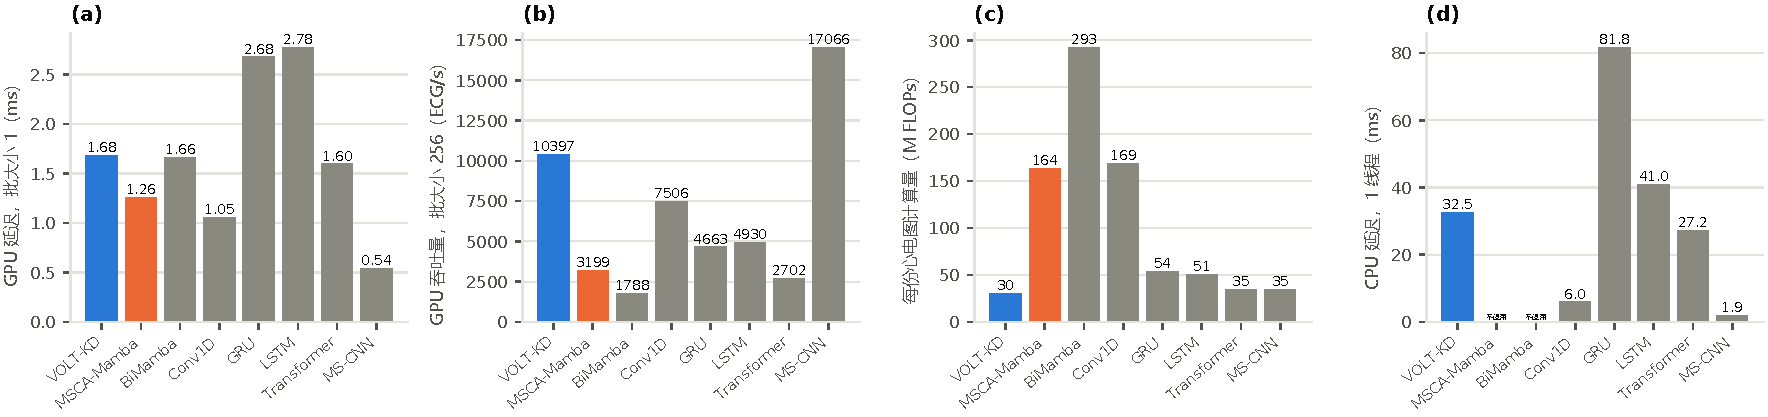
\includegraphics[width=\linewidth,height=0.45\textheight,keepaspectratio]{f15_efficiency.pdf}
\caption{八种结构在同一平台上的单条 GPU 延迟、批量吞吐、估计运算量与单线程 CPU 延迟。配置与测量单位见表。}\label{fig:efficiency}
\end{figure}

\section{讨论（Discussion）}
轻量心电图分类的有效容量取决于网络规模，也取决于预处理后仍可利用的诊断信息。MSCA-Mamba 等方法侧重多尺度特征提取与时序聚合\cite{cetintas2026}，本文则将幅值处理纳入同一设计过程。电压探针、两种骨干的输入对照和增益干预形成连续证据：毫伏表示保留肥厚相关电压统计量，这些信息可被紧凑网络利用，并参与最终预测。相对于既有幅值处理认识\cite{nolin2026}，本研究进一步量化了其在约十万参数分类器中的收益及类别分布，确立了输入信息保留对资源受限学习的实际价值。

输入设计、结构压缩和知识学习在 VOLT-KD 中承担不同作用。幅值保留产生主要排序收益，深度可分离卷积与短序列处理降低运算量，教师概率在固定学生规模下改善宏平均 F1。无 GRU 和宽度减半变体仍保持较高 AUC，进一步表明本文性能并不以增加时序模块复杂度为前提。教师—学生比较中的小幅 AUC 差距与显著参数规模差距说明，训练期监督和部署期容量可以分离；HYP 上的蒸馏退化则要求知识迁移兼顾学生已有的类别优势。按类别组织蒸馏权重，并评价保留毫伏输入的教师，是检验这一权衡的直接方向。

内部亚组、测试扰动和减导联结果从不同条件检验了这一设计。完整方法的收益覆盖多个测试人群及设备分组，并在所测噪声范围内保持；减导联训练则表明，统一骨干可以适应不同观测集合，但更少导联伴随可用诊断信息减少。幅值响应同时要求采集增益与毫伏换算一致。当前结论基于 PTB-XL 短时记录及心电图读图标签，外部数据库和真实采集设备评价将进一步检验跨来源适用性。输入对照包含中心化、尺度处理及对应增强的联合变化，教师方案包含微调样本量差异；预处理析因实验和匹配微调数据的教师对照可进一步分离这些操作的作用。

\section{结论（Conclusion）}
本文提出幅值保留的轻量多标签心电图分类框架 VOLT-KD，将毫伏输入、多尺度紧凑表征与训练期分层知识学习结合。电压探针和两个骨干的对照表明，幅值保留是分类性能改善的主要来源，其收益集中体现于肥厚相关类别。完整模型以 107,189 个部署参数达到宏平均 ROC-AUC 0.9298，教师监督进一步提高宏平均 F1，并呈现可辨识的类别权衡。计算评估显示，该设计降低估计运算量并提高批量吞吐。研究为轻量心电图分类提供了从诊断信息、训练监督到部署资源的连贯设计依据。

\section*{数据可用性}
PTB-XL 1.0.3 可通过 PhysioNet 获取：\url{https://physionet.org/content/ptb-xl/1.0.3/}。本文使用的逐种子结果、统计汇总与配置记录由研究项目保存。

\begin{thebibliography}{99}
\bibitem{wagner2020} Wagner P, Strodthoff N, Bousseljot RD, et al. PTB-XL, a large publicly available electrocardiography dataset. \emph{Scientific Data}. 2020;7:154. \url{https://doi.org/10.1038/s41597-020-0495-6}.

\bibitem{cetintas2026} Cetintas D. MSCA-Mamba: A Compact Multi-Scale Mamba Network for Multi-Label ECG Classification. \emph{Diagnostics}. 2026;16(19):3135. \url{https://doi.org/10.3390/diagnostics16193135}.

\bibitem{behrouz2024} Behrouz A, Santacatterina M, Zabih R. Chimera: Effectively Modeling Multivariate Time Series with 2-Dimensional State Space Models. \emph{Advances in Neural Information Processing Systems}. 2024;37:119886--119918. \url{https://proceedings.neurips.cc/paper_files/paper/2024/hash/d8e80772c27beff4ae1676fb147bbf26-Abstract-Conference.html}.

\bibitem{feng2025} Feng N, Chen C, Du P, Gong C, Pei J, Huang D. MS-LTCAF: A Multi-Scale Lead-Temporal Co-Attention Framework for ECG Arrhythmia Detection. \emph{Bioengineering}. 2025;12(9):1007. \url{https://doi.org/10.3390/bioengineering12091007}.

\bibitem{luo2025} Luo K, Huang L, He H, Chen Y, You L, Chen S, Chen J, Liu C. Efficient and Interpretable ECG Abnormality Detection via a Lightweight DSCR-BiGRU-Attention Network with Demographic Fusion. \emph{Mathematics}. 2025;13(23):3882. \url{https://doi.org/10.3390/math13233882}.

\bibitem{malik2026} Malik A, Aras S. A lightweight hybrid framework integrating convolutional neural networks and fast Fourier transform for reliable and calibrated ECG-based cardiac abnormality detection. \emph{PLOS One}. 2026;21(7):e0354834. \url{https://doi.org/10.1371/journal.pone.0354834}.

\bibitem{sokolow1949} Sokolow M, Lyon TP. The ventricular complex in left ventricular hypertrophy as obtained by unipolar precordial and limb leads. \emph{American Heart Journal}. 1949;37(2):161--186. \url{https://doi.org/10.1016/0002-8703(49)90562-1}.

\bibitem{casale1985} Casale PN, Devereux RB, Kligfield P, et al. Electrocardiographic detection of left ventricular hypertrophy: development and prospective validation of improved criteria. \emph{Journal of the American College of Cardiology}. 1985;6(3):572--580. \url{https://doi.org/10.1016/S0735-1097(85)80115-7}.

\bibitem{hancock2009} Hancock EW, Deal BJ, Mirvis DM, et al. AHA/ACCF/HRS Recommendations for the Standardization and Interpretation of the Electrocardiogram: Part V: Electrocardiogram Changes Associated With Cardiac Chamber Hypertrophy. \emph{Journal of the American College of Cardiology}. 2009;53(11):992--1002. \url{https://doi.org/10.1016/j.jacc.2008.12.015}.

\bibitem{nolin2026} Nolin-Lapalme A, Sowa A, Delfrate J, et al. Foundation models for electrocardiogram interpretation: clinical implications. \emph{European Heart Journal}. 2026;47(18):2174--2186. \url{https://doi.org/10.1093/eurheartj/ehaf1119}.

\bibitem{li2025} Li J, Aguirre AD, Moura V, et al. An Electrocardiogram Foundation Model Built on over 10 Million Recordings. \emph{NEJM AI}. 2025;2(7). \url{https://doi.org/10.1056/AIoa2401033}.

\bibitem{mckeen2025} McKeen K, Masood S, Toma A, Rubin B, Wang B. ECG-FM: an open electrocardiogram foundation model. \emph{JAMIA Open}. 2025;8(5):ooaf122. \url{https://doi.org/10.1093/jamiaopen/ooaf122}.

\bibitem{qin2023} Qin Y, Sun L, Chen H, Yang W, Zhang WQ, Fei J, Wang G. MVKT-ECG: Efficient single-lead ECG classification for multi-label arrhythmia by multi-view knowledge transferring. \emph{Computers in Biology and Medicine}. 2023;166:107503. \url{https://doi.org/10.1016/j.compbiomed.2023.107503}.

\bibitem{mehari2022} Mehari T, Strodthoff N. Self-supervised representation learning from 12-lead ECG data. \emph{Computers in Biology and Medicine}. 2022;141:105114. \url{https://doi.org/10.1016/j.compbiomed.2021.105114}.

\bibitem{vaid2023} Vaid A, Jiang J, Sawant A, et al. A foundational vision transformer improves diagnostic performance for electrocardiograms. \emph{npj Digital Medicine}. 2023;6:108. \url{https://doi.org/10.1038/s41746-023-00840-9}.

\bibitem{mert2026} Mert YE, Akdo\u{g}an E, \"{U}vet H. Multi-Label 12-Lead ECG Classification on the PTB-XL Dataset: A Comparative Evaluation of Deep Learning Architectures and Heterogeneous Ensemble Approaches. \emph{arXiv preprint}. 2026;2609.12803v1. \url{https://arxiv.org/abs/2609.12803}.

\bibitem{howard2017} Howard AG, Zhu M, Chen B, et al. MobileNets: Efficient Convolutional Neural Networks for Mobile Vision Applications. \emph{arXiv}. 2017;1704.04861. \url{https://arxiv.org/abs/1704.04861}.

\bibitem{cho2014} Cho K, van Merrienboer B, Gulcehre C, et al. Learning Phrase Representations using RNN Encoder--Decoder for Statistical Machine Translation. \emph{Proceedings of EMNLP}. 2014;1724--1734. \url{https://doi.org/10.3115/v1/D14-1179}.

\bibitem{hinton2015} Hinton G, Vinyals O, Dean J. Distilling the Knowledge in a Neural Network. \emph{arXiv}. 2015;1503.02531. \url{https://arxiv.org/abs/1503.02531}.

\bibitem{loshchilov2019} Loshchilov I, Hutter F. Decoupled Weight Decay Regularization. \emph{International Conference on Learning Representations}. 2019. \url{https://openreview.net/forum?id=Bkg6RiCqY7}.
\end{thebibliography}


\clearpage\appendix
\setcounter{table}{0}\renewcommand{\thetable}{S\arabic{table}}
\setcounter{figure}{0}\renewcommand{\thefigure}{S\arabic{figure}}
\section{补充方法与完整实验结果}
\subsection{对照实现与测量条件}
MSCA-Mamba 依据公开方法描述建立\cite{cetintas2026}：三路 $12\rightarrow32$ 通道卷积使用核 7、膨胀率 1/2/4、批归一化、ReLU 和压缩比 4 的 SE；拼接后的 96 通道通过 $1\times1$ 融合卷积、层归一化和单向 Mamba。Mamba 状态维度为 16、局部卷积核为 4、扩展倍数为 2。全局平均与最大池化后连接 $192\rightarrow128\rightarrow64\rightarrow5$ 分类头，参数量为 121,149。融合层与分类头宽度依据参数约束确定；序列块与分类头 dropout 分别设为 0.1 和 0.3，为本文实现取值。

本地 MSCA-Mamba 的输入对照采用相同网络和训练设置。毫伏配置使用中位数中心化，z-score 配置使用均值中心化与标准差缩放；VOLT-KD 学生噪声增强的标准差为 0.01 个输入单位。ECGFounder 测试预测由四个留出教师的 logits 平均得到，每个教师约含 30.69 百万参数；学生训练记录的软标签由对应的留出教师单独生成。

效率测量在 NVIDIA GB10 上进行，GPU 延迟在预热后重复 500 次，吞吐率使用批量 256；CPU 测量使用单线程。计时对象为模型前向推理，存储和内存使用 MiB。训练辅助头在学生部署测量中删除。教师训练成本属于训练阶段开销。


\subsection{数据结构与电压探针完整数值}
PTB-XL 中的诊断大类存在共现，同一记录可对应多个阳性目标（图\ref{fig:dataset}）。独立二元分类头和多标签损失使 VOLT-KD 能够保留这些共存关系。开发数据与测试折的电压探针均在毫伏表示下获得较高 ROC-AUC（表\ref{tab:voltage}），支持幅值相关信息并非只出现在单一测试分折中。
\begin{figure}[htbp]
\centering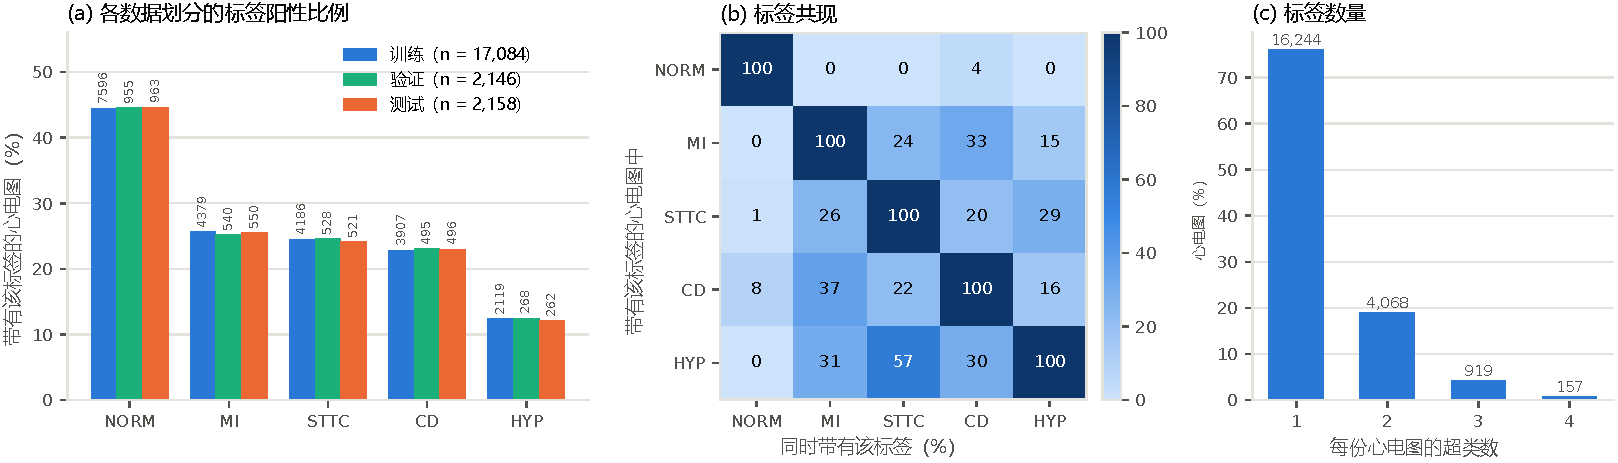
\includegraphics[width=\linewidth,height=0.40\textheight,keepaspectratio]{f01_dataset.pdf}
\caption{诊断大类分布、共现关系与标签数量。分折保持患者独立，标签允许共现。}\label{fig:dataset}
\end{figure}

\begin{table}[htbp]
\centering
\footnotesize
\caption{无需训练的电压探针在开发数据与测试折上的 ROC-AUC。开发数据指训练与验证折。}
\label{tab:voltage}
\begin{tabular}{lllrrr}
\toprule
数据 & 目标 & 指标 & 阳性数 & 毫伏 & z-score \\
\midrule
测试折 & HYP & Sokolow-Lyon & 262 & \textbf{0.786} & 0.527 \\
测试折 & HYP & Cornell & 262 & \textbf{0.702} & 0.582 \\
测试折 & LVH & Sokolow-Lyon & 214 & \textbf{0.876} & 0.591 \\
测试折 & LVH & Cornell & 214 & \textbf{0.745} & 0.614 \\
开发数据 & HYP & Sokolow-Lyon & 2387 & \textbf{0.809} & 0.500 \\
开发数据 & HYP & Cornell & 2387 & \textbf{0.705} & 0.543 \\
开发数据 & LVH & Sokolow-Lyon & 1918 & \textbf{0.894} & 0.573 \\
开发数据 & LVH & Cornell & 1918 & \textbf{0.723} & 0.576 \\
\bottomrule
\end{tabular}
\end{table}
\subsection{训练过程与逐类预测行为}
VOLT-KD 与本地 MSCA-Mamba 的五种子验证轨迹见图\ref{fig:training}，检查点均由验证集选择。完整 VOLT-KD 的逐类 ROC、精确率—召回率曲线及验证阈值下的混淆矩阵分别见图\ref{fig:roc}、图\ref{fig:pr}和图\ref{fig:confusion}，六项逐类指标见表\ref{tab:class}。这些结果同时刻画各类别的排序能力与阈值决策，避免以单一宏平均指标掩盖类别间的差异。
\begin{figure}[htbp]
\centering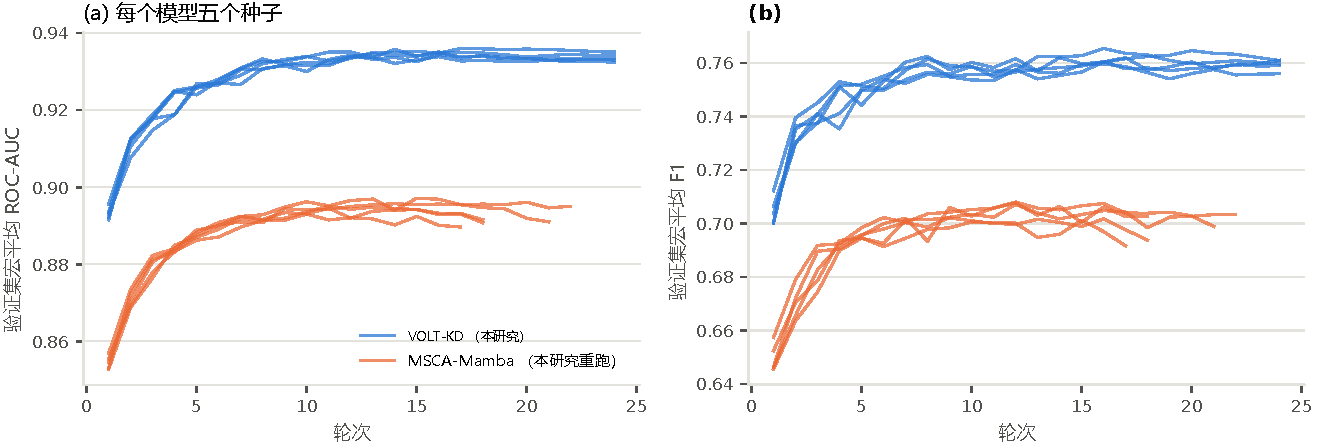
\includegraphics[width=\linewidth,height=0.32\textheight,keepaspectratio]{f04_training_curves.pdf}
\caption{完整 VOLT-KD 与本地 MSCA-Mamba 的验证集宏平均 ROC-AUC 和宏平均 F1 训练轨迹，每个模型包含五个随机种子。}\label{fig:training}
\end{figure}

\begin{table}[htbp]
\centering\footnotesize
\setlength{\tabcolsep}{3pt}
\caption{完整 VOLT-KD 的逐类结果，五种子均值与标准差；粗体标出每列在五个类别中的最高均值。}\label{tab:class}
\begin{tabularx}{\linewidth}{Yrrrrrr}
\toprule
类别 & ROC-AUC & AP & F1 & 精确率 & 召回率 & 特异度 \\
\midrule
NORM & $\boldsymbol{0.951\pm0.001}$ & $\boldsymbol{0.932\pm0.002}$ & $\boldsymbol{0.864\pm0.004}$ & $0.801\pm0.016$ & $\boldsymbol{0.938\pm0.012}$ & $0.812\pm0.021$ \\
MI & $0.937\pm0.002$ & $0.860\pm0.005$ & $0.768\pm0.004$ & $0.737\pm0.017$ & $0.801\pm0.023$ & $0.902\pm0.012$ \\
STTC & $0.942\pm0.002$ & $0.837\pm0.006$ & $0.779\pm0.004$ & $0.741\pm0.028$ & $0.823\pm0.030$ & $0.908\pm0.016$ \\
CD & $0.925\pm0.003$ & $0.859\pm0.004$ & $0.768\pm0.008$ & $\boldsymbol{0.835\pm0.017}$ & $0.712\pm0.023$ & $\boldsymbol{0.958\pm0.006}$ \\
HYP & $0.895\pm0.002$ & $0.650\pm0.011$ & $0.592\pm0.008$ & $0.575\pm0.054$ & $0.619\pm0.065$ & $0.935\pm0.020$ \\
\bottomrule
\end{tabularx}

\end{table}

\begin{figure}[htbp]
\centering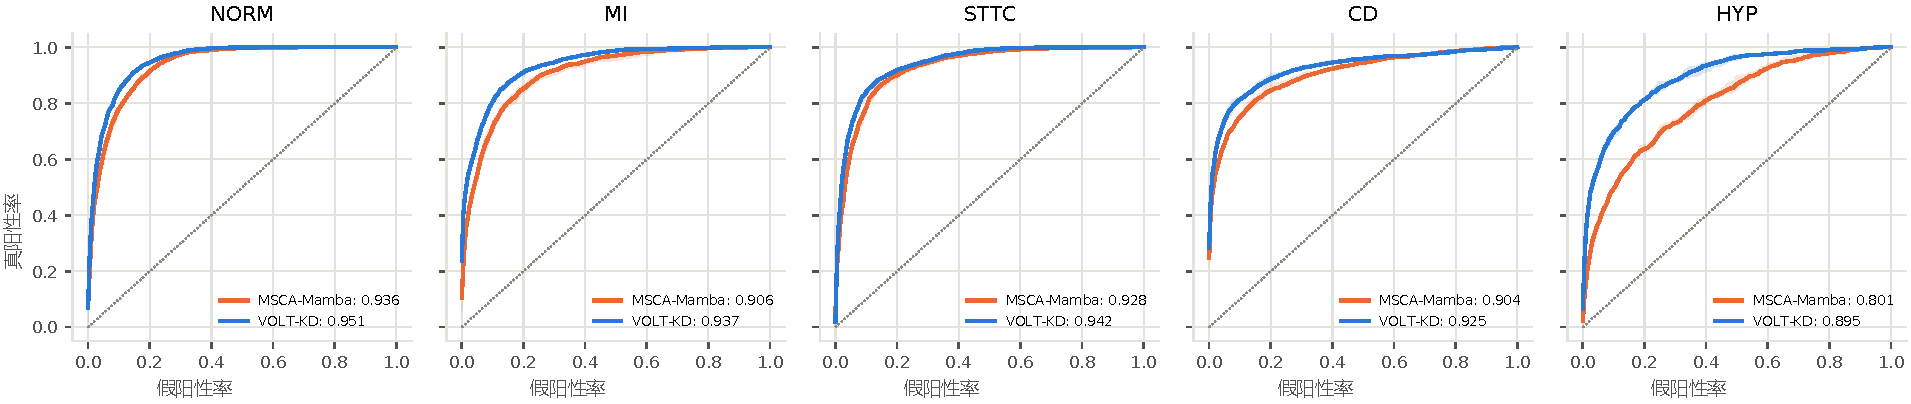
\includegraphics[width=\linewidth,height=0.33\textheight,keepaspectratio]{f08_roc.pdf}
\caption{完整 VOLT-KD 与本地 MSCA-Mamba 的五类 ROC 曲线。实线为五种子平均，阴影为各运行曲线的范围。}\label{fig:roc}
\end{figure}

\begin{figure}[htbp]
\centering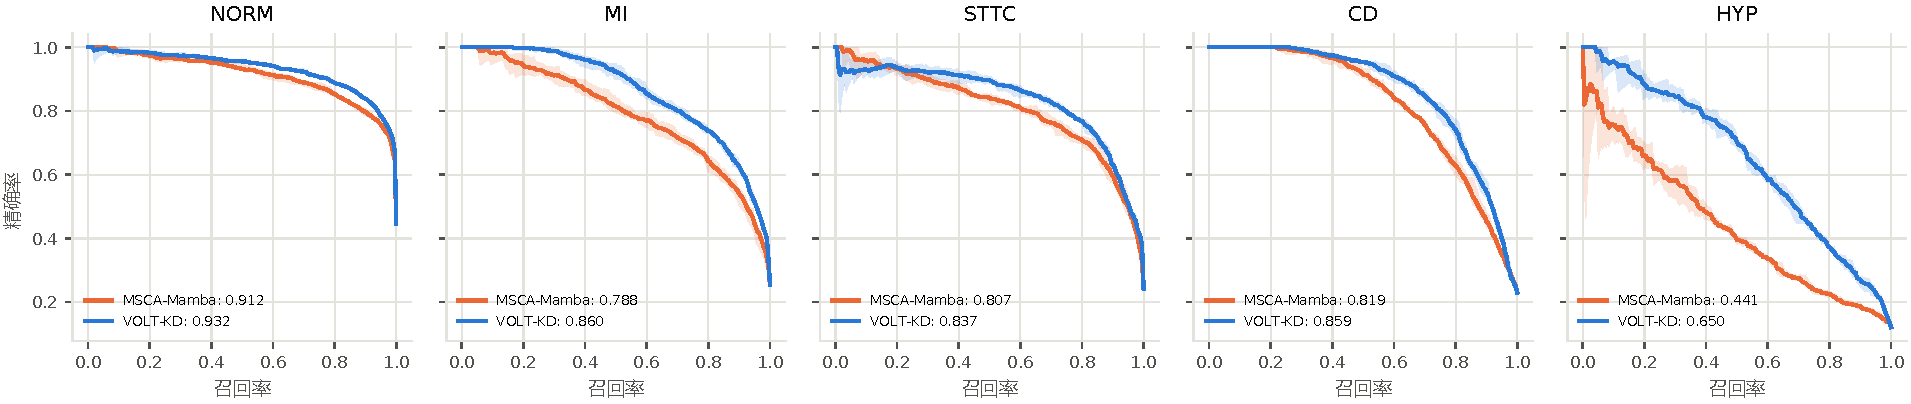
\includegraphics[width=\linewidth,height=0.33\textheight,keepaspectratio]{f09_pr.pdf}
\caption{完整 VOLT-KD 与本地 MSCA-Mamba 的五类精确率—召回率曲线。}\label{fig:pr}
\end{figure}

\begin{figure}[htbp]
\centering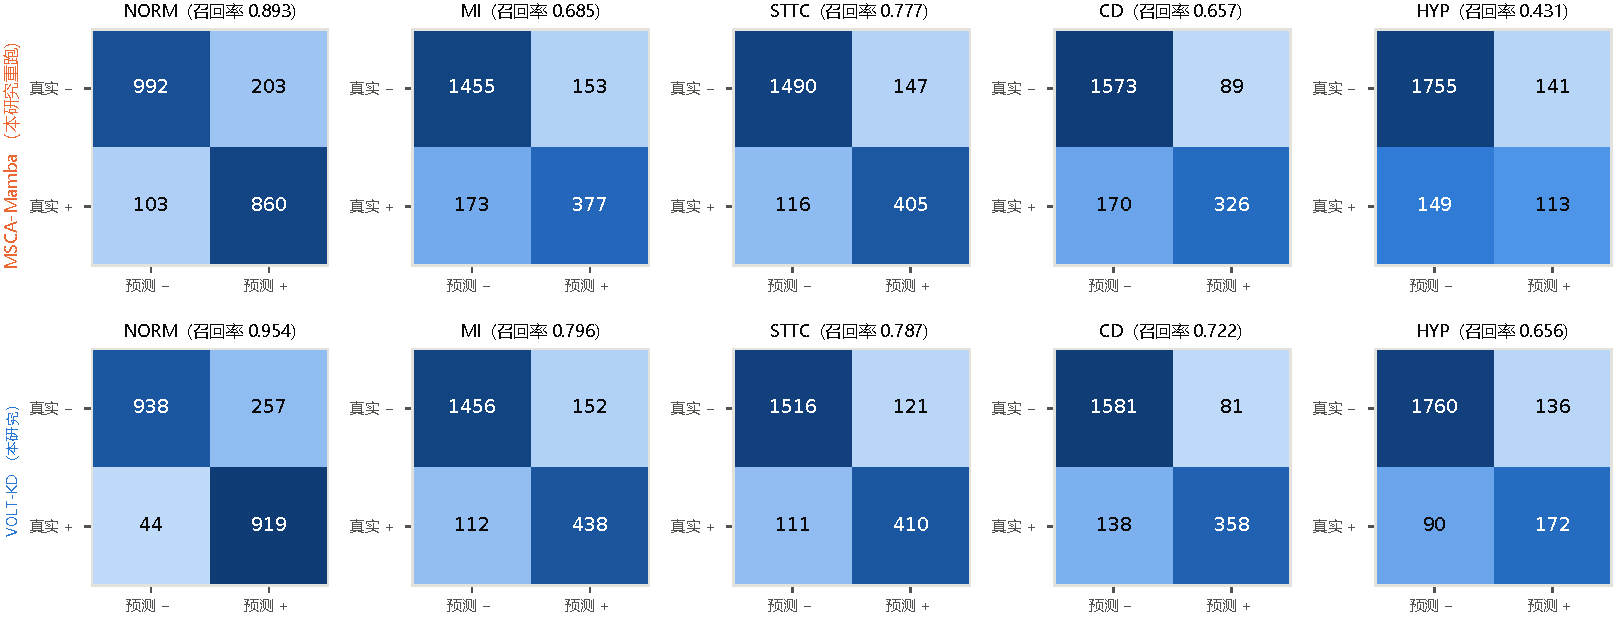
\includegraphics[width=\linewidth,height=0.51\textheight,keepaspectratio]{f10_confusion.pdf}
\caption{本地 MSCA-Mamba 与 VOLT-KD 的种子 42 二元混淆矩阵。每个类别均使用验证集确定的阈值。}\label{fig:confusion}
\end{figure}

\subsection{文献配置与逐种子比较的补充证据}
VOLT-KD 相对 MSCA-Mamba 文献九种配置的 45 项均值差均为正（图\ref{fig:vsall}）。对照覆盖卷积、循环、状态空间与注意力结构，支持本文在这一紧凑配置集合中的整体性能优势。区间由双方报告的标准差近似构造，统计对象为种子运行汇总，未合并文献与本地的病例级预测。
\begin{figure}[htbp]
\centering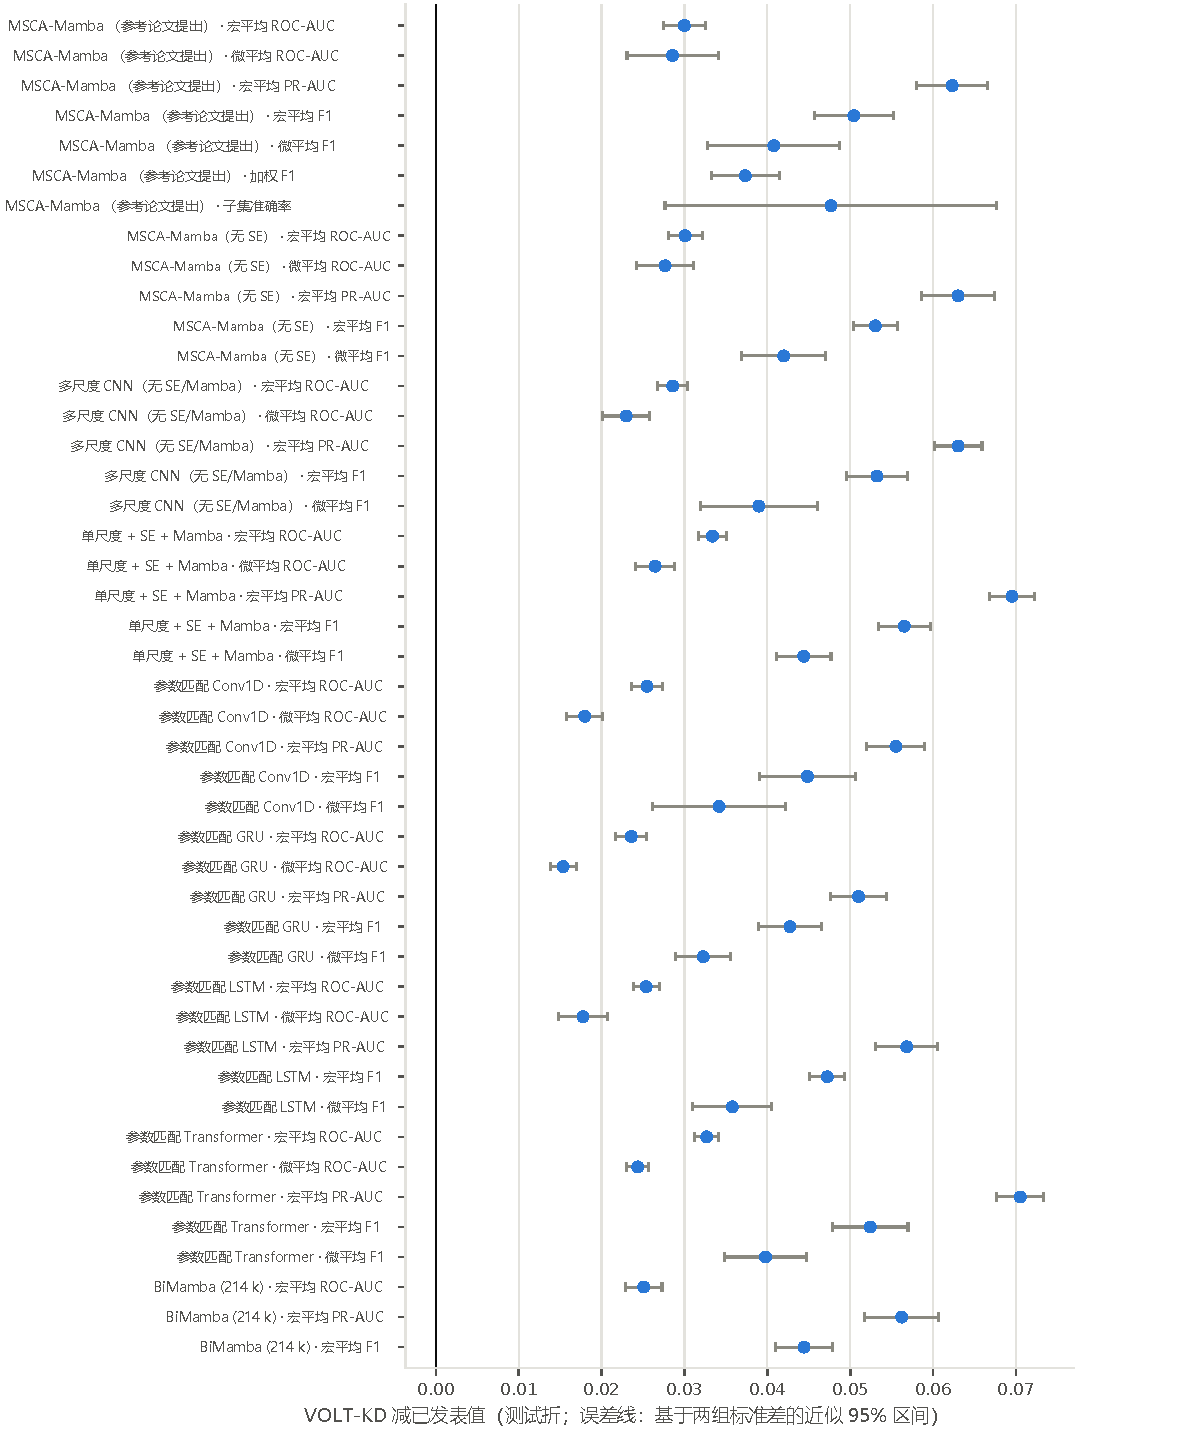
\includegraphics[width=\linewidth,height=0.86\textheight,keepaspectratio]{f06_vs_published.pdf}
\caption{相对于 MSCA-Mamba 原论文九种配置的 45 项报告均值差\cite{cetintas2026}。原文数值与本文值对应相同指标，点为本文减文献，误差线为报告标准差构造的近似区间。}\label{fig:vsall}
\end{figure}

表\ref{tab:paired_full}分别估计训练随机性与测试样本变化带来的不确定性。种子配对 $t$ 区间采用共同种子的指标差，记录级 bootstrap 区间采用 1,000 次测试记录重采样。蒸馏相对已有子类监督的宏平均 F1 增量为 0.0043，种子区间为 [0.0022, 0.0064]，记录重采样区间为 [$-0.0012$, 0.0100]。该差异支持固定测试集上多次训练的 F1 改善，其样本层面的增量仍随重采样而变化。bootstrap 检验同时报告 Holm 校正结果。
\begin{table}[htbp]
\centering\footnotesize
\caption{完整 VOLT-KD 减本地对照配置的配对结果。除 MSCA-Mamba 外，各行均为 VOLT-KD 骨干的消融配置；AUC、AP 和 F1 均为宏平均指标。}\label{tab:paired_full}
\begin{tabularx}{\linewidth}{Ylrrrr}
\toprule
对照配置 & 指标 & 差值 & 95\% 种子区间 & 95\% 记录区间 & $p_{\mathrm{Holm}}$ \\
\midrule
MSCA-Mamba 本地 & AUC & +0.0348 & [+0.0328, +0.0368] & [+0.0301, +0.0396] & 0.091 \\
MSCA-Mamba 本地 & AP & +0.0738 & [+0.0695, +0.0782] & [+0.0624, +0.0844] & 0.091 \\
MSCA-Mamba 本地 & F1 & +0.0602 & [+0.0568, +0.0635] & [+0.0506, +0.0693] & 0.091 \\
仅大类监督，z-score & AUC & +0.0192 & [+0.0170, +0.0214] & [+0.0158, +0.0229] & 0.091 \\
仅大类监督，z-score & AP & +0.0480 & [+0.0439, +0.0521] & [+0.0376, +0.0572] & 0.091 \\
仅大类监督，z-score & F1 & +0.0353 & [+0.0310, +0.0396] & [+0.0279, +0.0431] & 0.091 \\
仅大类监督，毫伏 & AUC & +0.0020 & [+0.0012, +0.0029] & [+0.0002, +0.0037] & 1.000 \\
仅大类监督，毫伏 & AP & +0.0036 & [+0.0002, +0.0071] & [-0.0013, +0.0081] & 1.000 \\
仅大类监督，毫伏 & F1 & +0.0058 & [+0.0034, +0.0082] & [+0.0002, +0.0110] & 1.000 \\
大类与子类监督 & AUC & +0.0017 & [-0.0003, +0.0038] & [+0.0001, +0.0032] & 1.000 \\
大类与子类监督 & AP & +0.0034 & [-0.0017, +0.0085] & [-0.0009, +0.0072] & 1.000 \\
大类与子类监督 & F1 & +0.0043 & [+0.0022, +0.0064] & [-0.0012, +0.0100] & 1.000 \\
完整监督 z-score & AUC & +0.0119 & [+0.0103, +0.0134] & [+0.0089, +0.0151] & 0.091 \\
完整监督 z-score & AP & +0.0325 & [+0.0279, +0.0372] & [+0.0230, +0.0415] & 0.091 \\
完整监督 z-score & F1 & +0.0259 & [+0.0232, +0.0286] & [+0.0186, +0.0331] & 0.091 \\
去除子类目标 & AUC & -0.0001 & [-0.0021, +0.0019] & [-0.0011, +0.0008] & 1.000 \\
去除子类目标 & AP & -0.0000 & [-0.0027, +0.0027] & [-0.0024, +0.0025] & 1.000 \\
去除子类目标 & F1 & +0.0024 & [-0.0013, +0.0061] & [-0.0018, +0.0061] & 1.000 \\
样本内教师 & AUC & -0.0006 & [-0.0012, -0.0001] & [-0.0019, +0.0004] & 1.000 \\
样本内教师 & AP & -0.0008 & [-0.0032, +0.0017] & [-0.0039, +0.0018] & 1.000 \\
样本内教师 & F1 & -0.0018 & [-0.0079, +0.0043] & [-0.0060, +0.0018] & 1.000 \\
noisy-OR 头 & AUC & -0.0008 & [-0.0016, +0.0000] & [-0.0021, +0.0005] & 1.000 \\
noisy-OR 头 & AP & -0.0019 & [-0.0137, +0.0099] & [-0.0051, +0.0015] & 1.000 \\
noisy-OR 头 & F1 & +0.0008 & [-0.0039, +0.0055] & [-0.0040, +0.0063] & 1.000 \\
去除 GRU & AUC & -0.0001 & [-0.0007, +0.0005] & [-0.0014, +0.0013] & 1.000 \\
去除 GRU & AP & -0.0019 & [-0.0045, +0.0006] & [-0.0051, +0.0011] & 1.000 \\
去除 GRU & F1 & +0.0004 & [-0.0053, +0.0061] & [-0.0055, +0.0056] & 1.000 \\
半宽学生 & AUC & +0.0004 & [-0.0039, +0.0048] & [-0.0008, +0.0017] & 1.000 \\
半宽学生 & AP & -0.0016 & [-0.0188, +0.0157] & [-0.0052, +0.0016] & 1.000 \\
半宽学生 & F1 & -0.0039 & [-0.0137, +0.0059] & [-0.0092, +0.0011] & 1.000 \\
\bottomrule
\end{tabularx}

\end{table}

VOLT-KD 的 noisy-OR 分类头、无 GRU 层和宽度减半变体采用三个共同种子，其余配置采用五个共同种子。bootstrap 以记录为重采样单位，未聚合同一患者的多条记录；配对分析作为探索性效应估计。
\subsection{完整子类与分组结果}
二十一个诊断子类的父类检出比例见表\ref{tab:subclass}。LVH、AMI、IMI、IRBBB 和 AVB 的改善表明，完整 VOLT-KD 的多标签收益能够覆盖若干具体诊断形态；不同子类的样本量和收益差异仍予保留。人口、设备和记录条件分组采用同一测试折（表\ref{tab:subgroup}），区间由各组内 300 次记录重采样得到。人工验证标签覆盖全部测试记录。
\begin{table}[htbp]
\centering\footnotesize
\caption{完整 VOLT-KD 与本地 MSCA-Mamba 在诊断子类记录中的父类检出比例。至少五条记录，五种子均值；差值由未舍入结果计算。}\label{tab:subclass}
\begin{tabularx}{\linewidth}{Ylrrrr}
\toprule
父类 & 子类 & 记录数 & 本地对照 & VOLT-KD & 差值 \\
\midrule
CD & LAFB/LPFB & 179 & \textbf{0.834} & 0.829 & -0.004 \\
CD & IRBBB & 112 & 0.714 & \textbf{0.805} & +0.091 \\
CD & AVB & 82 & 0.527 & \textbf{0.644} & +0.117 \\
CD & IVCD & 79 & \textbf{0.327} & 0.289 & -0.038 \\
CD & CLBBB & 54 & \textbf{0.993} & 0.989 & -0.004 \\
CD & CRBBB & 54 & \textbf{1.000} & \textbf{1.000} & +0.000 \\
CD & ILBBB & 8 & \textbf{0.850} & 0.750 & -0.100 \\
CD & WPW & 8 & \textbf{0.500} & 0.450 & -0.050 \\
HYP & LVH & 214 & 0.595 & \textbf{0.721} & +0.125 \\
HYP & LAO/LAE & 42 & 0.310 & \textbf{0.362} & +0.052 \\
HYP & RVH & 12 & 0.133 & \textbf{0.250} & +0.117 \\
HYP & RAO/RAE & 10 & 0.120 & \textbf{0.160} & +0.040 \\
MI & IMI & 327 & 0.765 & \textbf{0.826} & +0.061 \\
MI & AMI & 306 & 0.801 & \textbf{0.854} & +0.054 \\
MI & LMI & 20 & \textbf{0.380} & 0.360 & -0.020 \\
NORM & NORM & 963 & 0.899 & \textbf{0.938} & +0.040 \\
STTC & STTC & 222 & 0.765 & \textbf{0.766} & +0.001 \\
STTC & ISC & 128 & 0.925 & \textbf{0.953} & +0.028 \\
STTC & ISCA & 93 & 0.832 & \textbf{0.869} & +0.037 \\
STTC & NST & 77 & 0.779 & \textbf{0.803} & +0.023 \\
STTC & ISCI & 40 & 0.775 & \textbf{0.800} & +0.025 \\
\bottomrule
\end{tabularx}

\end{table}

\begin{table}[htbp]
\centering\footnotesize
\caption{本文完整 VOLT-KD 学生模型与本地 MSCA-Mamba 对照模型的测试亚组比较。数值为宏平均 ROC-AUC 的五种子均值及记录级 bootstrap 区间；差值为完整 VOLT-KD 减本地 MSCA-Mamba。}\label{tab:subgroup}
\begin{tabularx}{\linewidth}{Yrrrr}
\toprule
分组 & 记录数 & \shortstack{MSCA-Mamba\\（本地对照）} & \shortstack{VOLT-KD\\（完整模型）} & 差值 \\
\midrule
全部记录 & 2158 & 0.895 [0.887, 0.904] & \textbf{0.930} [0.922, 0.936] & +0.035 \\
男性 & 1110 & 0.906 [0.895, 0.916] & \textbf{0.940} [0.931, 0.947] & +0.034 \\
女性 & 1048 & 0.884 [0.871, 0.896] & \textbf{0.920} [0.909, 0.930] & +0.036 \\
年龄 $<40$ & 284 & 0.894 [0.857, 0.925] & \textbf{0.930} [0.905, 0.952] & +0.035 \\
年龄 40--59 & 639 & 0.893 [0.874, 0.911] & \textbf{0.922} [0.901, 0.940] & +0.030 \\
年龄 60--74 & 706 & 0.882 [0.867, 0.896] & \textbf{0.925} [0.913, 0.936] & +0.043 \\
年龄 $\geq75$ & 529 & 0.859 [0.840, 0.880] & \textbf{0.906} [0.890, 0.919] & +0.047 \\
无噪声标记 & 1645 & 0.897 [0.888, 0.907] & \textbf{0.932} [0.925, 0.939] & +0.035 \\
有噪声标记 & 513 & 0.887 [0.865, 0.902] & \textbf{0.923} [0.906, 0.937] & +0.036 \\
单一大类 & 1650 & 0.855 [0.840, 0.871] & \textbf{0.920} [0.907, 0.931] & +0.065 \\
多个大类 & 508 & 0.852 [0.838, 0.865] & \textbf{0.896} [0.884, 0.908] & +0.044 \\
设备: CS-12 & 686 & 0.859 [0.843, 0.877] & \textbf{0.900} [0.886, 0.915] & +0.040 \\
设备: CS-12   E & 437 & 0.891 [0.863, 0.917] & \textbf{0.929} [0.908, 0.946] & +0.038 \\
设备: AT-6 C 5.5 & 382 & 0.907 [0.893, 0.924] & \textbf{0.947} [0.934, 0.958] & +0.040 \\
设备: AT-6     6 & 236 & 0.905 [0.882, 0.930] & \textbf{0.944} [0.924, 0.958] & +0.039 \\
\bottomrule
\end{tabularx}

\end{table}

\subsection{扰动强度与减导联完整结果}
十八种测试扰动的宏平均 AUC 及标准差见表\ref{tab:noise_full}。输入噪声在毫伏尺度施加，两种模型随后执行各自预处理。减导联训练中，十二导联缩减为六肢体导联时，MI 和 HYP 的 AUC 下降较大（表\ref{tab:leadclass}和图\ref{fig:leads}），与胸导联提供的形态及电压信息有关。该类别差异说明，导联压缩的代价取决于诊断任务所需的观测方向，不能仅由导联数量概括。
\begin{table}[htbp]
\centering\footnotesize
\caption{本文完整 VOLT-KD 学生模型与本地 MSCA-Mamba 对照模型在多强度测试扰动下的宏平均 ROC-AUC。数值为五种子均值与标准差，对应图\ref{fig:noise}；两种模型的训练参数保持固定。}\label{tab:noise_full}
\begin{tabularx}{\linewidth}{Yrrr}
\toprule
扰动 & 强度 & \shortstack{MSCA-Mamba\\（本地对照）} & \shortstack{VOLT-KD\\（完整模型）} \\
\midrule
基线漂移（mV） & 0 & $0.8950\pm0.0024$ & $\boldsymbol{0.9298\pm0.0012}$ \\
基线漂移（mV） & 0.1 & $0.8808\pm0.0033$ & $\boldsymbol{0.9291\pm0.0012}$ \\
基线漂移（mV） & 0.2 & $0.8507\pm0.0077$ & $\boldsymbol{0.9262\pm0.0014}$ \\
基线漂移（mV） & 0.5 & $0.7309\pm0.0125$ & $\boldsymbol{0.9058\pm0.0037}$ \\
基线漂移（mV） & 1 & $0.5973\pm0.0104$ & $\boldsymbol{0.8032\pm0.0080}$ \\
基线漂移（mV） & 2 & $0.5230\pm0.0099$ & $\boldsymbol{0.6070\pm0.0081}$ \\
高斯噪声（mV） & 0 & $0.8950\pm0.0024$ & $\boldsymbol{0.9298\pm0.0012}$ \\
高斯噪声（mV） & 0.01 & $0.8949\pm0.0023$ & $\boldsymbol{0.9296\pm0.0012}$ \\
高斯噪声（mV） & 0.02 & $0.8937\pm0.0021$ & $\boldsymbol{0.9296\pm0.0011}$ \\
高斯噪声（mV） & 0.05 & $0.8841\pm0.0018$ & $\boldsymbol{0.9291\pm0.0009}$ \\
高斯噪声（mV） & 0.1 & $0.8499\pm0.0058$ & $\boldsymbol{0.9236\pm0.0011}$ \\
高斯噪声（mV） & 0.2 & $0.7720\pm0.0125$ & $\boldsymbol{0.8976\pm0.0041}$ \\
导联置零 & 0 & $0.8950\pm0.0024$ & $\boldsymbol{0.9298\pm0.0012}$ \\
导联置零 & 1 & $0.8853\pm0.0027$ & $\boldsymbol{0.9200\pm0.0015}$ \\
导联置零 & 2 & $0.8714\pm0.0038$ & $\boldsymbol{0.9105\pm0.0018}$ \\
导联置零 & 4 & $0.8315\pm0.0045$ & $\boldsymbol{0.8823\pm0.0010}$ \\
导联置零 & 6 & $0.7678\pm0.0091$ & $\boldsymbol{0.8315\pm0.0027}$ \\
导联置零 & 8 & $0.6763\pm0.0147$ & $\boldsymbol{0.7491\pm0.0084}$ \\
\bottomrule
\end{tabularx}

\end{table}

\begin{table}[htbp]
\centering\footnotesize
\caption{VOLT-KD 学生不同导联配置的逐类 ROC-AUC。完整十二导联模型采用五种子，分别训练的减导联变体采用三个种子。}\label{tab:leadclass}
\begin{tabularx}{\linewidth}{Yrrrrr}
\toprule
输入 & NORM & MI & STTC & CD & HYP \\
\midrule
十二导联 & $\boldsymbol{0.951\pm0.001}$ & $\boldsymbol{0.937\pm0.002}$ & $\boldsymbol{0.942\pm0.002}$ & $\boldsymbol{0.925\pm0.003}$ & $\boldsymbol{0.895\pm0.002}$ \\
六肢体导联 & $0.929\pm0.000$ & $0.888\pm0.003$ & $0.922\pm0.001$ & $0.896\pm0.004$ & $0.848\pm0.000$ \\
仅 II 导联 & $0.904\pm0.002$ & $0.827\pm0.001$ & $0.885\pm0.002$ & $0.877\pm0.003$ & $0.790\pm0.002$ \\
\bottomrule
\end{tabularx}

\end{table}

\begin{figure}[htbp]
\centering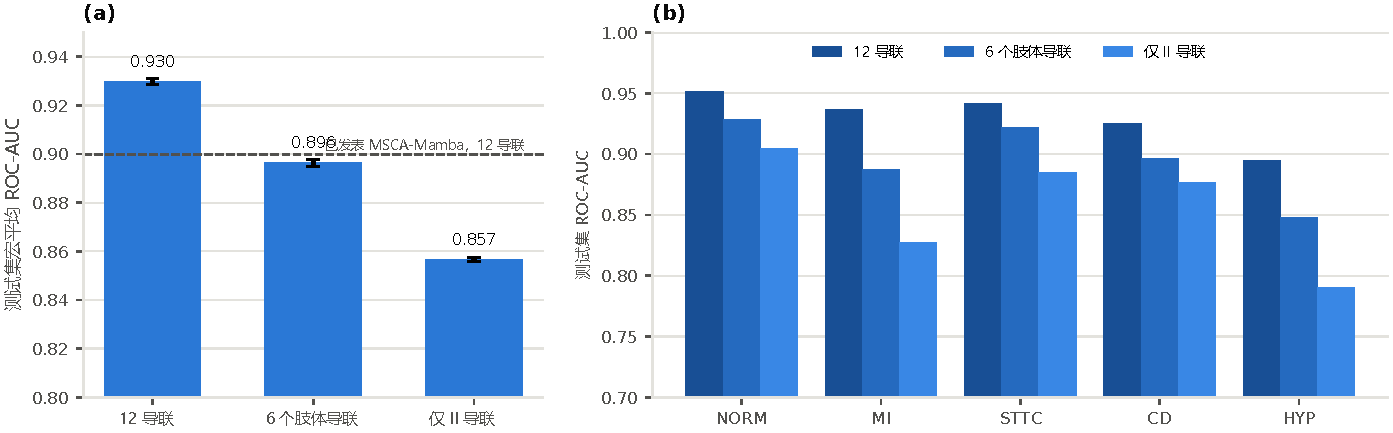
\includegraphics[width=\linewidth,height=0.36\textheight,keepaspectratio]{f21_reduced_leads.pdf}
\caption{本文 VOLT-KD 完整模型（十二导联）与六肢体导联、仅 II 导联学生变体的整体及逐类表现。三种配置均使用十二导联 ECGFounder 教师软标签，整体指标对应表\ref{tab:leads}。}\label{fig:leads}
\end{figure}

\subsection{集成、参数配置与局部归因}
表\ref{tab:ensemble}比较单模型均值与五种子概率集成。VOLT-KD 集成的宏平均 AUC 和 AP 分别达到 0.9326 和 0.8338，高于单模型平均的 0.9298 和 0.8274；宏平均 F1 分别为 0.7541 和 0.7542，完全匹配准确率分别为 0.6006 和 0.6168。集成主要改善预测排序，各种阈值指标呈现不同变化。本文主配置保持单模型部署，集成结果提供额外计算预算下的性能参照。
\begin{table}[htbp]
\centering\footnotesize
\caption{单模型与五种子概率集成。单模型行为五次独立运行的均值与标准差，集成行为单次联合评价；粗体分别标记单模型组和集成组的较高结果。}\label{tab:ensemble}
\begin{tabularx}{\linewidth}{Yrrrr}
\toprule
配置 & 宏平均 AUC & 宏平均 AP & 宏平均 F1 & 完全匹配 \\
\midrule
MSCA-Mamba，单模型均值 & $0.8950\pm0.0024$ & $0.7536\pm0.0033$ & $0.6941\pm0.0021$ & $0.5618\pm0.0219$ \\
MSCA-Mamba，五种子集成 & 0.9031 & 0.7713 & 0.7044 & 0.5820 \\
VOLT-KD，单模型均值 & $\boldsymbol{0.9298\pm0.0012}$ & $\boldsymbol{0.8274\pm0.0020}$ & $\boldsymbol{0.7542\pm0.0009}$ & $\boldsymbol{0.6168\pm0.0131}$ \\
VOLT-KD，五种子集成 & \textbf{0.9326} & \textbf{0.8338} & \textbf{0.7541} & \textbf{0.6006} \\
\bottomrule
\end{tabularx}

\end{table}

参数量与 AUC 的关系反映了输入设计和结构简化共同影响的资源权衡（图\ref{fig:pareto}）。图中的训练参数包含相应辅助分支，部署参数见表\ref{tab:efficiency}。图\ref{fig:saliency}呈现完整 VOLT-KD 种子 42 模型的五个高置信度正确示例，每类一条记录；梯度乘输入的符号表示局部信号对当前类别分数的一阶贡献方向。这些局部归因补充了模型利用波形的直观证据，其解释范围限于所展示记录。
\begin{figure}[htbp]
\centering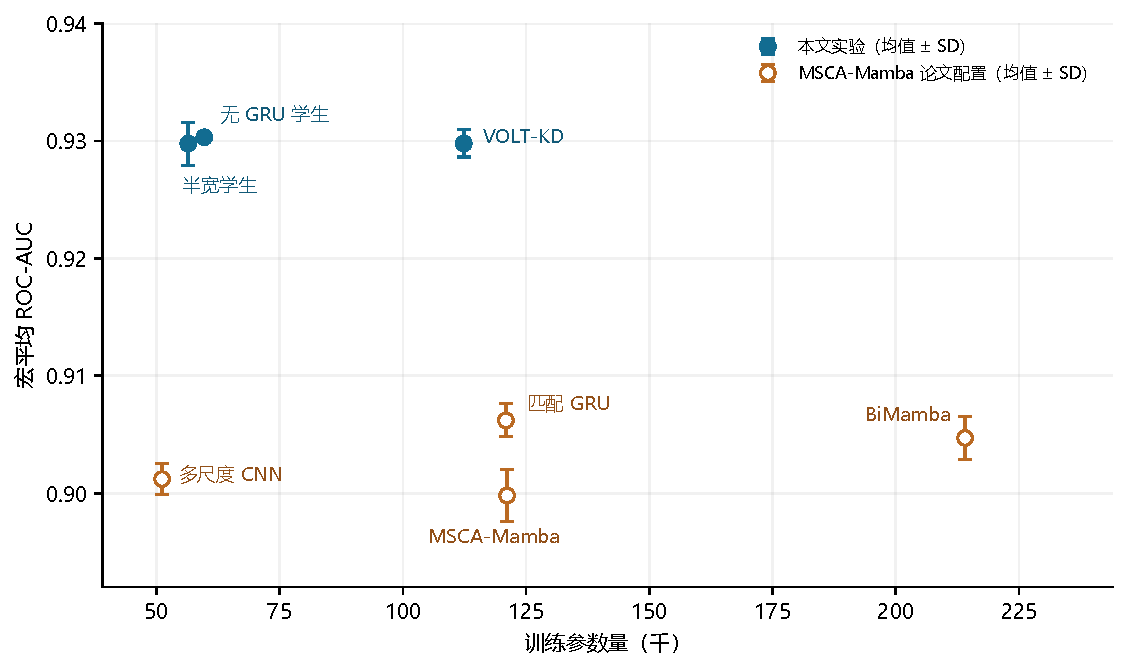
\includegraphics[width=\linewidth,height=0.45\textheight,keepaspectratio]{f14_pareto.pdf}
\caption{代表性紧凑配置的训练参数量与宏平均 ROC-AUC。实心点为本文完整学生、半宽与无 GRU 变体（分别为五、三、三个种子）；空心点为 MSCA-Mamba 原论文配置\cite{cetintas2026}，其余为本文实验配置。}\label{fig:pareto}
\end{figure}

\begin{figure}[htbp]
\centering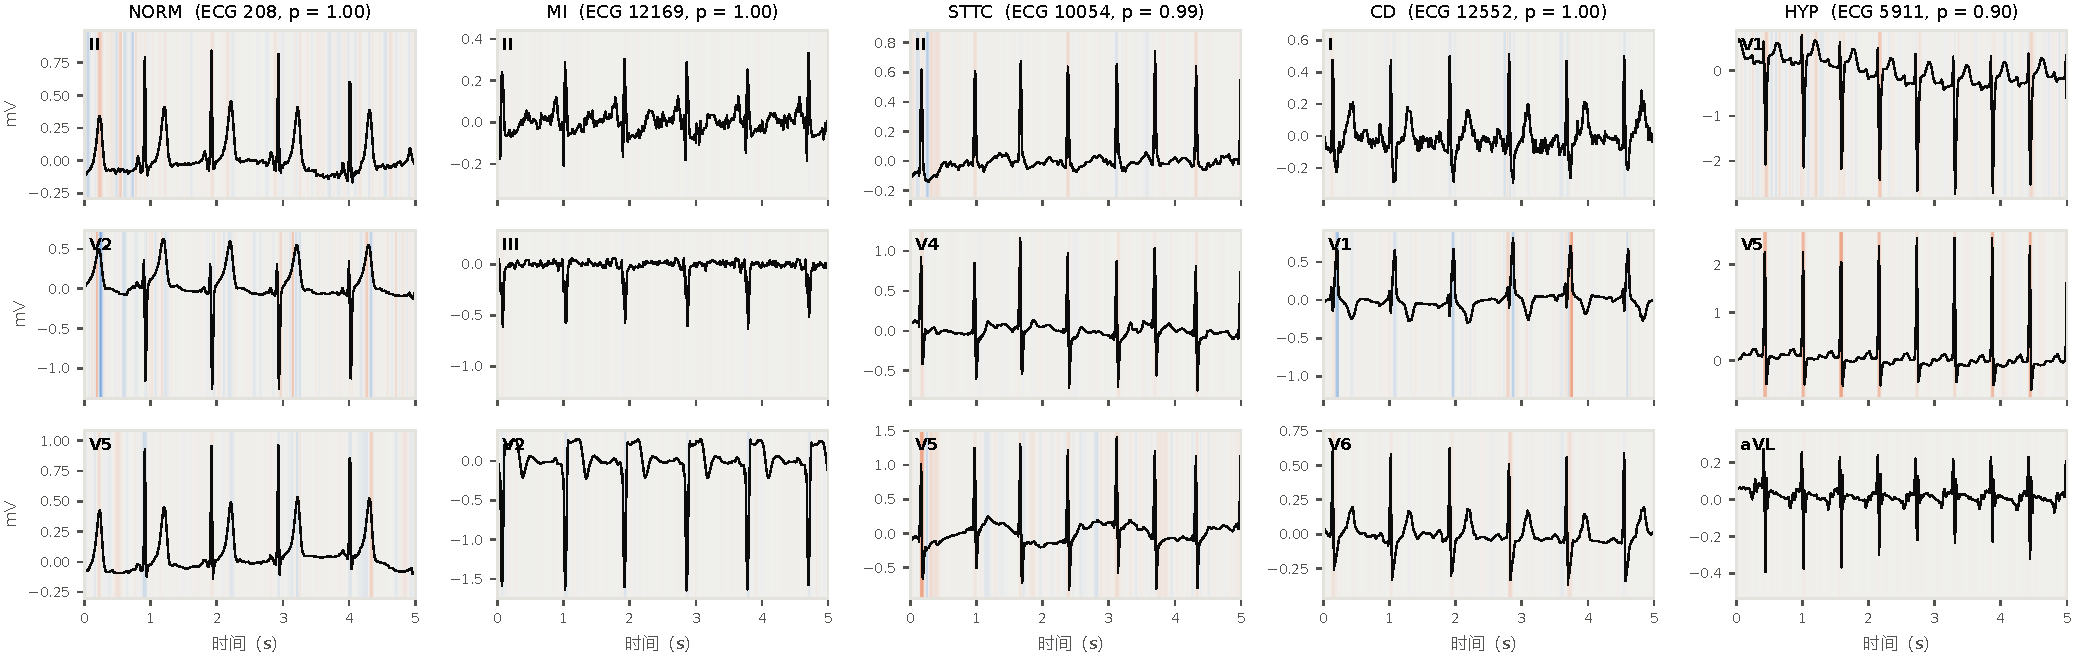
\includegraphics[width=\linewidth,height=0.72\textheight,keepaspectratio]{f23_attribution.pdf}
\caption{完整 VOLT-KD 的梯度乘输入局部归因示例，每类选取一条正确识别的种子 42 测试记录，显示三个导联。橙色和蓝色分别表示对类别分数的正、负贡献。}\label{fig:saliency}
\end{figure}

\subsection{扩展文献参照}
扩展文献比较涵盖不同的信息与计算资源配置（表\ref{tab:resource_refs}）。Chimera 建模多变量时间序列，DBA-ASFNet 融合波形与人口信息，CNN--FFT 结合时域与频域特征；ECGFounder 微调使用 500 Hz 输入，异构 stacking 组合多个推理模型。VOLT-KD 将基础模型知识用于训练，并以约十万参数的 100 Hz 单学生部署。各方法在输入信息、训练知识和推理路径上的差异，决定了其精度与资源权衡的不同位置，文献值按原作者协议报告。
\begin{table}[htbp]
\centering\footnotesize
\caption{扩展文献比较。除 VOLT-KD 外均为原作者报告值；参数单位为百万（M），粗体标出本表各项最优报告值。}\label{tab:resource_refs}
\begin{tabularx}{\linewidth}{Yc p{1.65cm} rrrr}
\toprule
方法与来源 & 年份 & 输入 & 参数 & \shortstack{宏平均\\ROC-AUC} & \shortstack{PR-AUC\\/AP} & \shortstack{宏平均\\F1} \\
\midrule
Chimera\cite{behrouz2024} & 2024 & 100 Hz & -- & 0.930 & -- & -- \\
DBA-ASFNet\cite{luo2025} & 2025 & 100 Hz+人口信息 & $\boldsymbol{\sim0.030}$ & 0.9166 & -- & -- \\
CNN--FFT\cite{malik2026} & 2026 & 500 Hz & 0.0869 & 0.9246 & 0.813 & \textbf{0.770} \\
ECGFounder 微调\cite{mert2026} & 2026 & 500 Hz & -- & 0.930 & 0.823 & 0.749 \\
异构 stacking\cite{mert2026} & 2026 & 多模型 & -- & \textbf{0.936} & \textbf{0.836} & 0.763 \\
VOLT-KD（本文） & -- & 100 Hz & 0.1072 & $0.9298\pm0.0012$ & $0.8274\pm0.0020$ & $0.7542\pm0.0009$ \\
\bottomrule
\end{tabularx}
\par\vspace{3pt}{\footnotesize Chimera 采用 NeurIPS 2024 正式版表 2 的 Superdiag 值；DBA-ASFNet 采用原文表 3 的 Super-Diag. 值，额外输入年龄与性别。CNN--FFT 为原论文的 500 Hz 五诊断大类结果。Mert 等的两项结果来自 2026 年预印本表 I，采用 PTB-XL 1.0.3 官方分折、单种子 42；本文为五种子均值与标准差。}
\end{table}

\subsection{统计与文献比较口径}
主文的种子配对区间由 $\bar d\pm t_{0.975,n-1}s_d/\sqrt n$ 计算。HYP 对宏平均 AUC 增量的算术贡献定义为 $\Delta\mathrm{AUC}_{\mathrm{HYP}}/(5\Delta\mathrm{AUC}_{\mathrm{macro}})$，用于说明等权汇总中类别增量的来源。所有本地检查点和阈值通过验证集选择。

文献比较保留原报告精度，数据版本、输入和重复运行设置见表\ref{tab:recent}和表\ref{tab:resource_refs}。MS-LTCAF 沿用原文 AUC/F1 名称，CNN--FFT 采用 0.5 阈值。
\end{document}
